
\section{Multivariate analysis}
\label{sec:mva}

From the cut-based analysis,
combining the significance of the three categories,
we obtain a signal significance of $S/\sqrt{B}\simeq 1.7 (3.5)$
with all backgrounds (only QCD $4b$) taken into account.
%
This is clearly
to be enough to be able to claim observation
of Higgs pair production
in this channel, and even less to extract the trilinear Higgs  coupling
$\lambda$, in particular
taking into account the that $S/B$ is at the permille level.
%
In this section we now show how this signal significance for
 can
be significance improved when
applying a multivariate analysis (MVA) subsequently
to the cut-based analysis.

 
%
Multivariate techniques are by now a mature tool to enhance signal
significance in HEP analysis, allowing
to open a new window to improve the performance
of many physics analysis and searches.
%
In particular, the classification of events as arising from either signal or
background processes via the use of a multivariate analysis is a
commonly applied strategy in LHC
applications~\cite{Baldi:2014pta,Aaltonen:2012qt,
  Wardrope:2014kya,Chatrchyan:2013zna,Dall'Osso:2015aia}.
%
For instance, the CMS $Vh(\to b\bar{b})$ analysis~\cite{Chatrchyan:2013zna}
is based on a Boosted Decision Tree (BDT) MVA, and the UCL $hh\to 4b$
feasibility study~\cite{Wardrope:2014kya}
also used  a BDT to improve signal discrimination.

In this section, first of all we present the specific MVA that we use,
based on feed-forward multi-layer neural networks.
%
We then introduce the input variables that are
used the MVA, including the jet substructure
variables, and then present the results of $S/\sqrt{B}$ including
the MVA effects.
%
Since we find that jet substructure variables are a crucial input
to the MVA, we finally show various kinematic distributions
of these variables.



\subsection{Deep artificial neural networks}


%
The specific type of  MVA that we use here, to
disentangle signal and background events in the $hh\to 4b$ process, will be
a multi-layer feed-forward artificial neural network (ANN),
also known as a {\it perceptron}.\footnote{This type of ANNs are the same
  as those used to parametrize Parton Distribution Functions
in the NNPDF global analyses~\cite{DelDebbio:2004qj,Ball:2008by,Ball:2011mu,Ball:2010de}.}
%
This family of ANNs is sometimes known as {\it deep} neural networks, since they have
a richer architecture with hidden layers.
%
The basic idea is that the ANN is trained on an input composed on
all  signal and background
events which satisfy the requirements of the
cut-based analysis.
%
The main result of the trained ANN is identifying, in a fully automated way,
which are the most relevant variables to discriminate between the two classes
of events.

In this work, the ANN that we use has the following architecture.
\be
\label{eq:nn1}
N_{\mathrm{var}}\times5\times3\times1 \, ,
\ee
where $N_{\mathrm{var}}$ represents the number of input variables for the MVA,
which is specific of the analysis category: resolved, intermediate, or boosted.
%
All neural-network layers use a sigmoid activation function, allowing
for a probabilistic
interpretation of the neural-network output.
%
In Fig.~\ref{fig:nnarch} we show an example of the ANN that we use in this work, corresponding here
to the case of the boosted category (thus $N_{\mathrm{var}}=21$, as we explain below).

%%%%%%%%%%%%%%%%%%%%%%%%
\begin{figure}[t]
  \begin{center}
      \vspace{-1cm}
  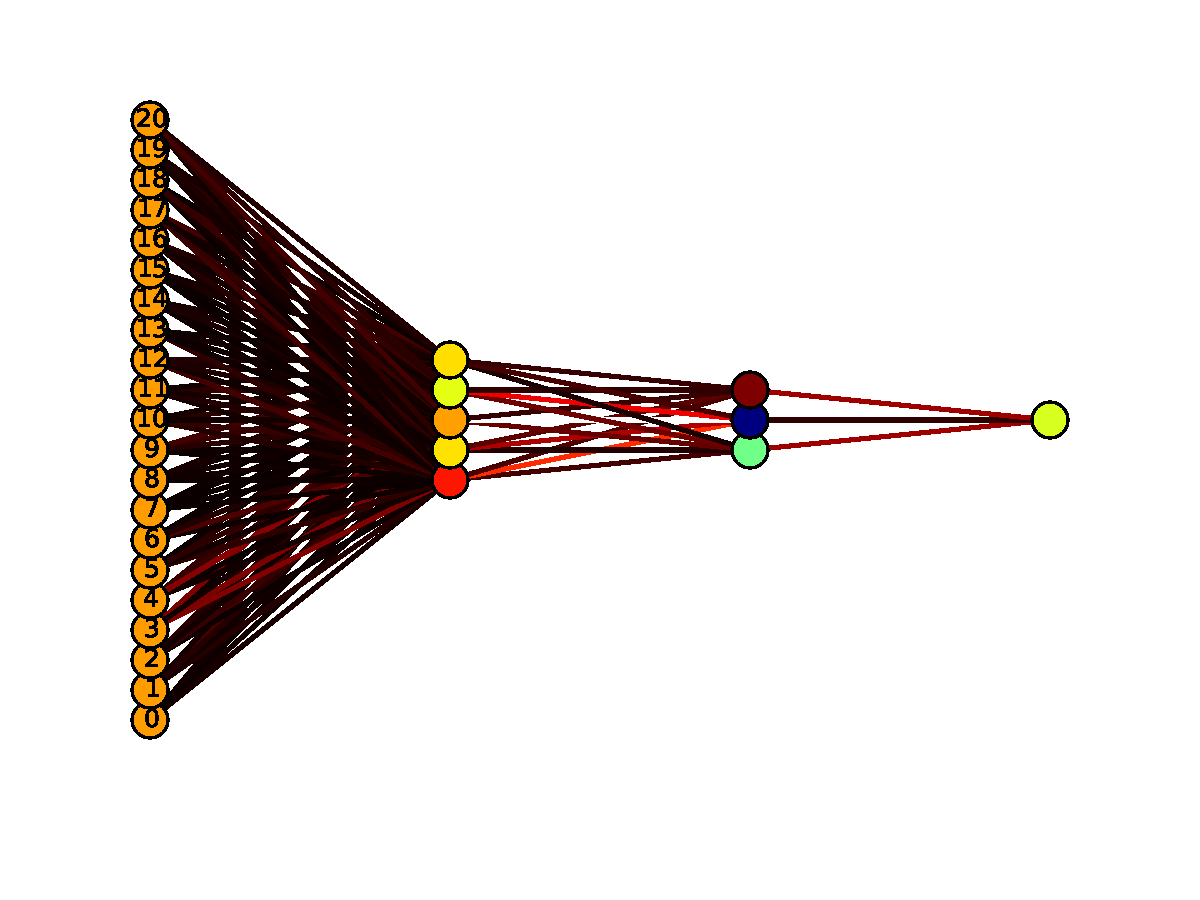
\includegraphics[width=0.90\textwidth]{plots/bst_nnarch_noPU.pdf}
  \vspace{-2cm}
  \caption{\small Architecture of the Artificial
    Neural Network (ANN)
    used for the analysis of the
    boosted
    category, with $N_{\rm var}=21$ input variables and thus
    the same number of neurons
  in the first layer.
  %
  The color code in the neuron connections (the weights) is a heat map,
  with red indicating large values and black small values.
}
\label{fig:nnarch}
\end{center}
\end{figure}
%%%%%%%%%%%%%%%%%%%%%%%

The training of the ANN for the signal/background classification task
proceeds as follows.
%
Given a set of $N_{\mathrm{var}}$  kinematic variables $\{k\}_i$ associated with the event $i$, and a set of neural network parameters $\{\omega\}$, we interpret the neural network output $y_i$ (that is, the activation state of the
neuron in the last layer)
as the probability that the event $i$ originates from the signal process,
\be
y_i = P(y^\prime_i=1|\{k\}_i, \{\omega\} )\, ,
\ee
where $y_i^\prime$ represents the true classification of the event $i$, i.e $y^\prime_{\text{signal}} = 1$ and $y^\prime_{\text{background}} = 0$. With this interpretation, our general classification probability including background events is given by
\be
P(y_i^\prime|\{k\}_i, \{\omega\}) = y_i^{y^\prime_i}(1-y_i)^{1-y^\prime_i} \, ,
\ee
which implies that the  negative log-likelihood cost function
that needs to be minimized during the ANN training is 
the cross-entropy error, defined as
 \bea
 E(\{\omega\}) &=& -\log\left(\prod_i^{N_{\text{evt}}} P(y_i^\prime|\{k\}_i, \{\omega\})\right)\nonumber\\
 &=&
 \sum_i^{N_{\text{evt}}} y^\prime_i\log{y_i} + (1-y^\prime_i)\log{(1-y_i)} \, ,
 \label{cross-entropy}
 \eea
 where $N_{\text{evt}}$ is the number of
 Monte Carlo events that we have generated.
 %
 The ANN is trained both on the signal and background MC events,
 in each case using the information $y_i'$ of the true nature
 of the event.
 %
 To be stable against statistical fluctuations, it is important to use
 a large enough MC sample both of signal and of background events
 for the MVA training.
 
 Therefore, the training of the neural networks consist on the
 minimization of the cross-entropy error,
 Eq.~(\ref{cross-entropy}), which in this work is achieved using a
 Genetic Algorithm.
 %
 The GA training is performed for a very large 
 number of generations, in this case $N_{\rm gen}=50k$, to avoid
 under-training.
 %
 We have verified that if a larger number of generations
 are used the results are unchanged.
 %

 In order to avoid over-fitting,
 we have used a cross-validation stopping
 criterion, in particular, the same one as
 that used in the NNPDF3.0 analysis~\cite{Ball:2014uwa}
 does not modify the results.
 %
 This cross-validation entails dividing the input MC dataset into two disjoint sets,
 and use one for the training and the other for the validation: the optimal
 stopping point is then indicated by the minimum of the error function
 Eq.~(\ref{cross-entropy}) for the validation sub-sample.

 

 \subsection{Input kinematical variables}
 \label{sec:input}

 To identify the variables with higher discriminatory power,
 we need to train
 the MVA using a large number of kinematic distributions for
 signal and background events.
%
In our $hh\to 4b$ case,
the input variables for the MVA differ between our three categories,
and in particular in the case of large-$R$ jets (for the boosted
and intermediate categories) we want to exploit
the richness of substructure information.

For the three categories, boosted, intermediate and resolved,
the following common variables are used as input to the MVA:
\begin{itemize}
\item The transverse momenta of the leading and subleading Higgs, $p_{T,h_1}$ and $p_{T,h_2}$.
\item The transverse momentum of the reconstructed Higgs pair, $p_{T,hh}$.
\item The invariant masses of the leading and sub-leading Higgs candidates, $m_{h,1}$ and $m_{h,2}$.
\item The invariant mass of the reconstructed Higgs pair, $m_{hh}$.
\item The separation in the $\phi$--$\eta$ plane
  between the two Higgs candidates, $\Delta R_{hh}$.
  \item The separation in $\eta$  between the two Higgs candidates, $\Delta \eta_{hh}$.
\item The separation in $\phi$  between the two Higgs candidates, $\Delta \phi_{hh}$.
\end{itemize}
In addition, in the boosted category we use
  the transverse momenta of the leading, $p_{T,h_{1,1}}$ and $p_{T,h_{1,2}}$ and
  sub-leading, $p_{T,h_{2,1}}$ and $p_{T,h_{2,1}}$, Higgs candidate subjets.
  %
  In the resolved category instead,
  the corresponding variables are
  the transverse momenta $p_{T,i}$ of the four leading 
  $b$-tagged small-$R$ jets in the event.
  %
  In the intermediate category, we use the
  transverse momenta of the subjets
  from the large-$R$ jet $p_{T,h_{1,1}}$ and $p_{T,h_{1,2}}$ and the
 transverse momenta $p_{T,i}$ of the two leading 
  $b$-tagged small-$R$ jets.
  %
Therefore, we have a total of 13 variables which are common to the three categories.
%
Therefore, there are in total $N_{\mathrm{var}}=13$ variables for the
resolved analysis,
17 for the intermediate,
and 21 for the boosted category.
%
Given that the MVA is able to identify the most discriminatory variables
and to ignore those that have smaller effect, it is advantageous to
include as many substructure variables as possible.
%
This is one of the main advantages of ANNs in this context: they are
inherently redundant, so
adding additional information, even if carries very little weight,
should not degrade
the classification power of the MVA (other than making the GA
minimization less efficient).

\subsection{Post-MVA signal significance}
\label{sec:signalsignificance}

In Fig.~\ref{fig:nnresponse} we show the distribution of
the ANN output at the end of the training, for the exclusive
boosted, intermediate and resolved categories.
%
The distributions are normalized so that their integral
  adds up to one.
%
The  separation between signal and background is achieving by introducing
a cut, $y_{\rm cut}$, in the ANN output, so that MC events with $y_i\ge
y_{\rm cut}$ are classified as signal events, and those with
 $y_i <
y_{\rm cut}$ as background events.
%
Therefore,
the more separated that the two distributions are, the more efficient
the MVA discrimination will be.



%%%%%%%%%%%%%%%%%%%%%%%%%%%%
\begin{figure}[t]
\begin{center}
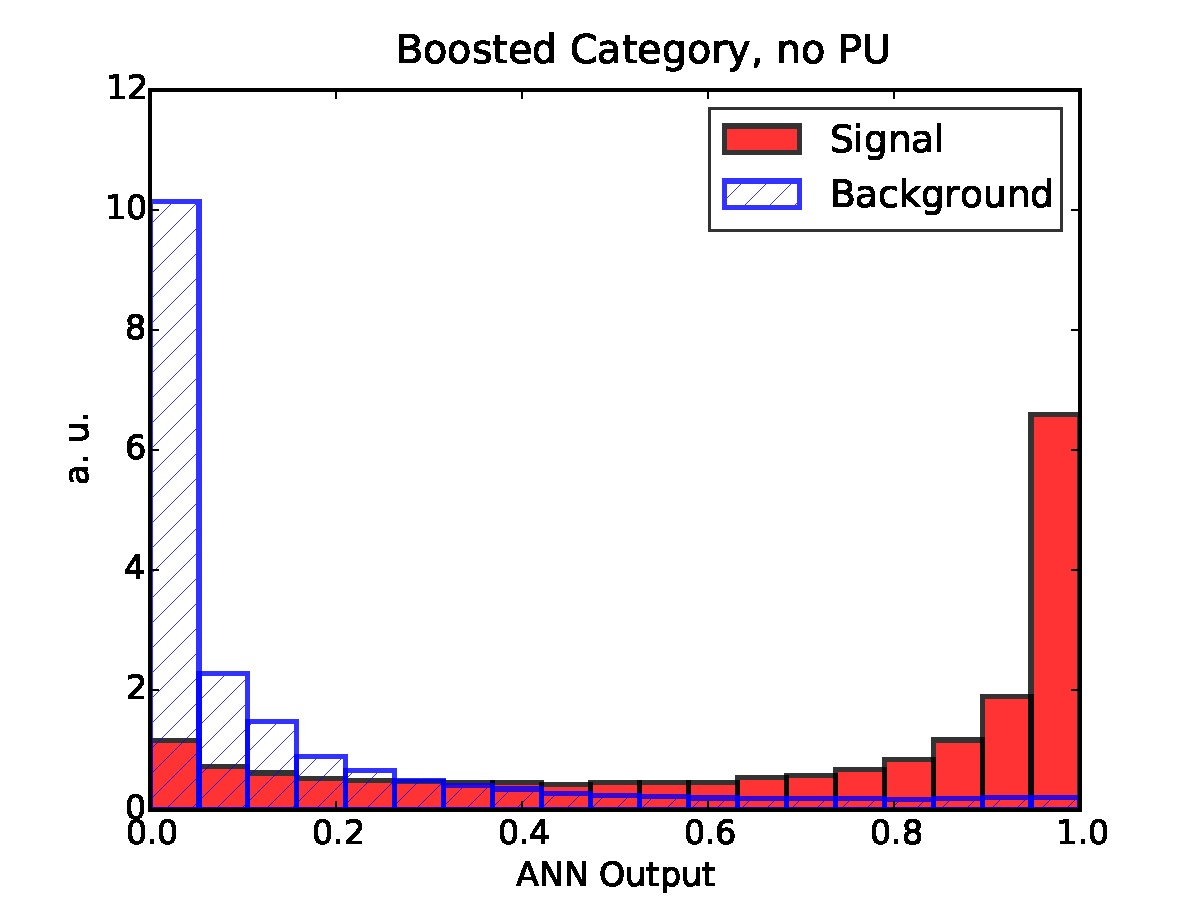
\includegraphics[width=0.65\textwidth]{plots/Boosted_disc_noPU.pdf}
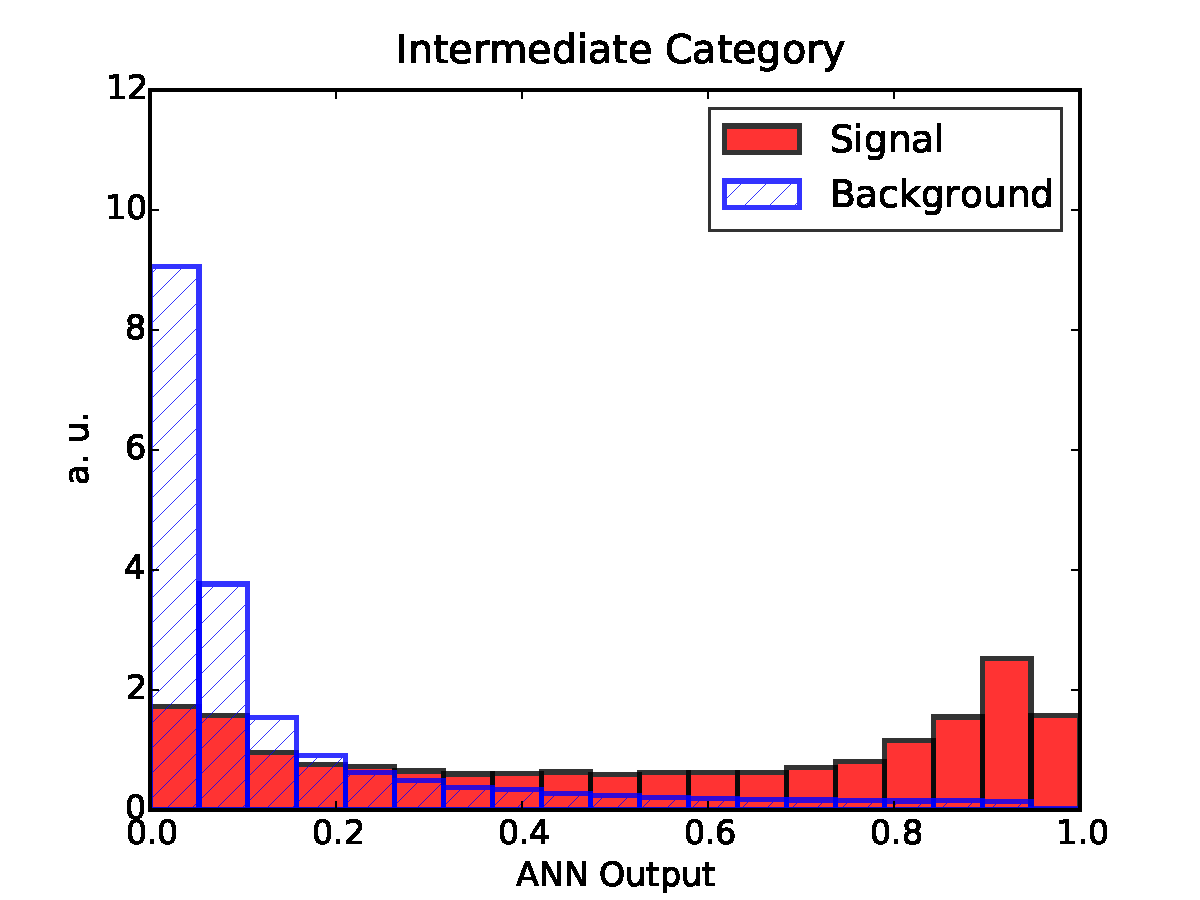
\includegraphics[width=0.48\textwidth]{plots/Intermediate_disc_noPU.pdf}
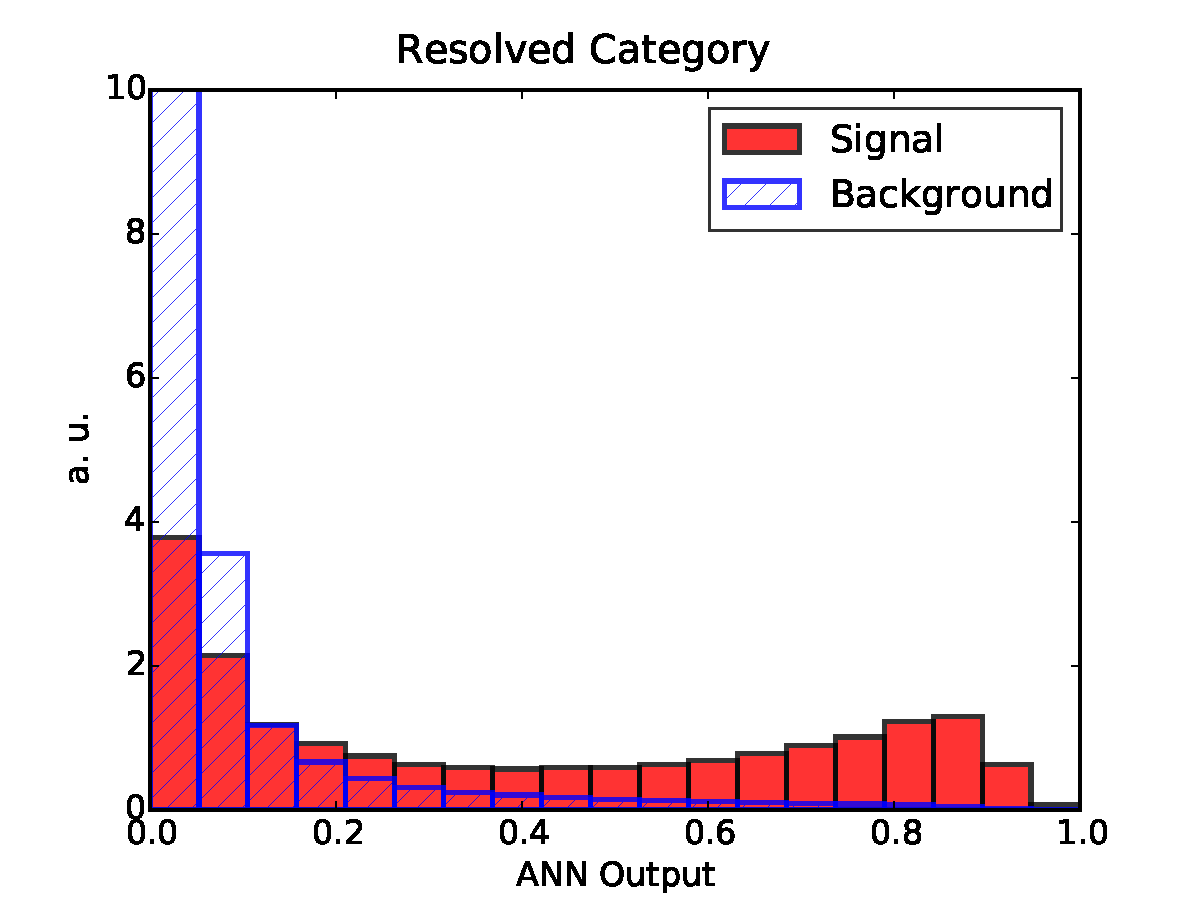
\includegraphics[width=0.48\textwidth]{plots/Resolved_disc_noPU.pdf}
\caption{\small The distributions, at the end of the
  GA training, 
  for the signal and background MC events in the three categories:
  boosted (upper plot), intermediate (lower left plot) and
  resolved (lower right plot), as a function of the ANN output.
  %
  All distributions are normalized so that their integrals
  add up to one.
}
\label{fig:nnresponse}
\end{center}
\end{figure}
%%%%%%%%%%%%%%%%%%%%%%%

From Fig.~\ref{fig:nnresponse} we see that in the boosted category the MVA manages
to achieve a clear discrimination between signal and background, with the two distributions
nicely peaking at 1 and at 0 respectively.
%
This indicates that introducing a suitable cut
$y_{\rm cut}$
in the ANN output will substantially reduce the background,
while keeping a reasonable signal efficiency.
%
The performance of the MVA discrimination is similar though slightly worse in the intermediate
category, and it is markedly worse in the resolved category.
%
We have traced back these differences to the use of jet substructure variables
in the boosted and intermediate categories, whose use substantially
improves the
discrimination between signal and background events.



The results for the signal selection efficiency and the 
background rejection rate as a function of the cut in the ANN output
$y_{\rm cut}$
define the so-called  Receiver-Operating Characteristic (ROC)
curve.
%
It is clear that we can achieve  high signal efficiency by using
a small value of the cut in the ANN output, but this choice will be
affected from a poor background
rejection.
%
Conversely, using a higher value of the cut will increase background rejection at the
cost of dropping signal efficiency.
%
Another important requirement on the value of $y_{\rm cut}$ is that
the  number of expected  signal events (the physical
events for a given integrated
luminosity, not the MC events used for the ANN training)
after the cut is large enough.

In Fig.~\ref{fig:exampleroc} the
we show the ROC curve for the background rejection rate as a function of the signal
  selection efficiency as the cut in the ANN output is varied.
  %
  We show the results for the three exclusive categories: boosted, intermediate
  and resolved.
%
As could already be inferred from the distribution of neural
networks output in Fig.~\ref{fig:nnresponse}, we find
that the neural network MVA is reasonably efficient
in discriminating signal over background.
%
The performance is best in the case of the boosted category,
decreasing then for the intermediate and finally for the
resolved categories, consistent with the distributions in
Fig.~\ref{fig:exampleroc}.
%



%%%%%%%%%%%%%%%%%%%%%%%%%%%%%%%%%%%%%%%%%%%%%%
\begin{figure}[t]
\begin{center}
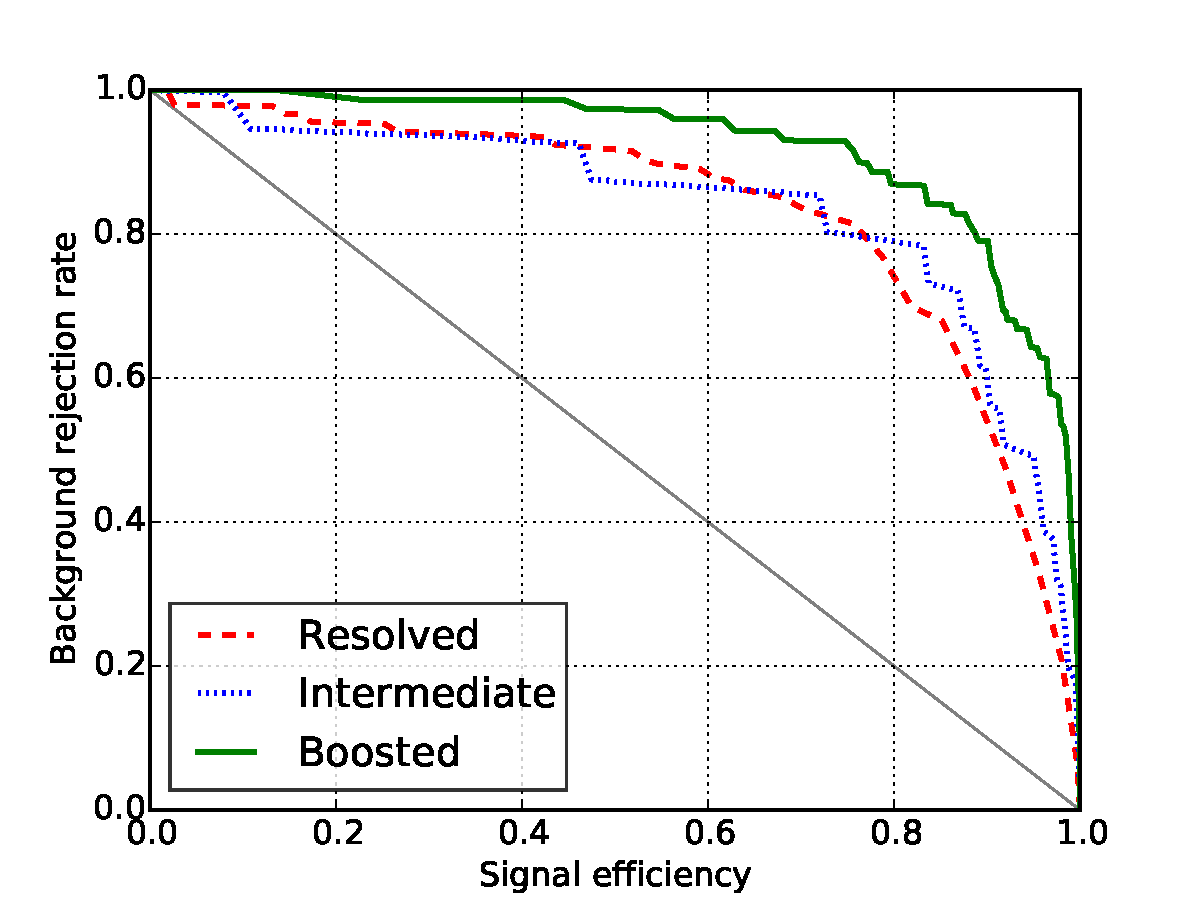
\includegraphics[width=0.65\textwidth]{plots/roc.pdf}
\caption{\small ROC curve for the background rejection rate as a function of the signal
  selection efficiency, as the cut in the ANN output is varied.
  %
  We show the results for the three exclusive categories: boosted, intermediate
  and resolved.
}
\label{fig:exampleroc}
\end{center}
\end{figure}
%%%%%%%%%%%%%%%%%%%%%%%%%%%%%%%%%%%%%

From Fig.~\ref{fig:exampleroc} we see that, always starting from the signal
and background events that survive the basic cut-based analysis,
one can achieve a  signal
efficiency of $\sim 90\%$ while reducing the background by
$80\%$, $60\%$ and $50\%$ in the boosted, intermediate and resolved
categories respectively.
%
It is easy to translate these factors into an  improvement factor of the pre-MVA
signal significance $S/\sqrt{B}$.
%
As an illustration, if a signal efficiency of 90\%
is required, we find that the MVA improves $S/\sqrt{B}$
by  approximately 2.0, 1.4 and 1.3  in the three categories respectively.

As mentioned above, an
 important restriction on the range of allowed cuts in the ANN output
 is that $y_{\rm cut}$
 cannot be so hard that the actual number of signal events expected
at the HL-LHC becomes unreasonably small.
%
To verify how many signal and background events are left after the MVA cut,
we show in Fig.~\ref{fig:nev2} the number of signal (dashed lines) and background (solid lines)
  events expected at the HL-LHC as a function of $y_{\rm cut}$,
  for the three exclusive categories.
  %
  Note that the value of the cut in the ANN cut is separately optimised in the three
  categories.

%%%%%%%%%%%%%%%%%%%%%%%%%%%%%%%%%%%%%%%%%%%%%%
\begin{figure}[t]
\begin{center}
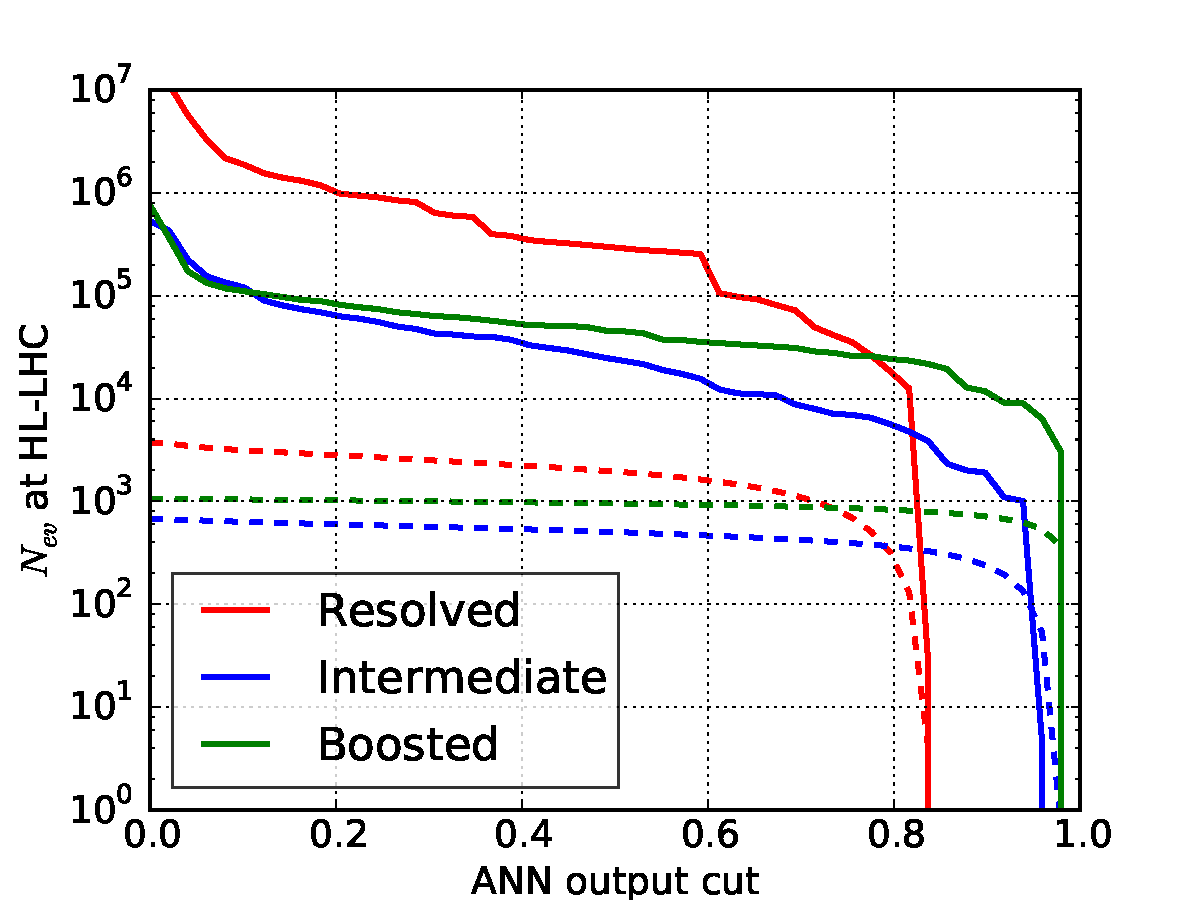
\includegraphics[width=0.65\textwidth]{plots/nev2_noPU.pdf}
\caption{\small Number of signal (dashed lines) and background (solid lines)
  events expected at the HL-LHC as a function of the cut in the ANN output,
  for the three separate categories.
}
\label{fig:nev2}
\end{center}
\end{figure}
%%%%%%%%%%%%%%%%%%%%%%%%%%%%%%%%%%%%%

As can be seen from Fig.~\ref{fig:nev2}, in the boosted category
event with a cut in the ANN output as hard as $y_{\rm cut}\simeq 0.9$
we are still left
with around 100 events at the HL-LHC, 
which the background being reduced substantially to around
1000 events.
%
A similar cut would work fine for the intermediate category, though here
the backgrounds are much larger and thus the expected signal significance smaller.
%
For the resolved case, the signal significance would be only slightly
improved for any value of the cut.

A useful property of MVAs such as the one used in this work
is that they provide direct  physical insight about which of the
input variables contribute the most to the separation of
signal over background.
%
In the case of ANNs, this can be quantified by computing the sum
of the absolute value of al the weights connected to a given
input neuron $i$, that is
\be
\label{eq:totweight}
\omega^{\rm tot}_i \equiv \sum_{k=1}^{n^{(2)}} \Big|\omega^{(2)}_{ki}\Big| \, ,
\qquad i=1,\ldots,N_{\rm var} \, ,
\ee
with $\omega^{(2)}_{ki}$ the value of the weight connecting
the $k$-th neutron of the second layer with the $i$-th neuron of
the first (input) layer, and $n^{(2)}=5$ the number of
neurons in the second layer.
%
The input variables with a larger value of $\omega^{\rm tot}_i$ will those
be the ones that play a dominant role in enhancing the signal
discrimination using the MVA.

%
In Fig.~\ref{fig:nnweights} we show
the distribution of the total associated weight,
Eq.~(\ref{eq:totweight}) for each of the $N_{\rm var}$ input
variables of the resolved (left plot) and boosted (right plot) categories.
%
The notation for the various kinematic variables is the same
as in Sect.~\ref{sec:input}.
%
The important information
is contained in the relative strengths of the total associated weight
for each of the input variables.
%
The results of Fig.~\ref{fig:nnweights} illustrate which variables
are more discriminative between the signal and the background.
%
For instance, in the 
resolved category, the variables that lead to
a higher discrimination power
are the $p_T$ of the two reconstructed Higgs candidates, and then on a similar
footing other variables like the $p_T$ of the individual jets
and the mass of the di-Higgs system $m_{hh}$.
%
The only variable which seems to contain to information at all
is the $\Delta \phi_{hh}$ separation between the two
Higgs candidates.


%%%%%%%%%%%%%%%%%%%%%%%%
\begin{figure}[t]
\begin{center}
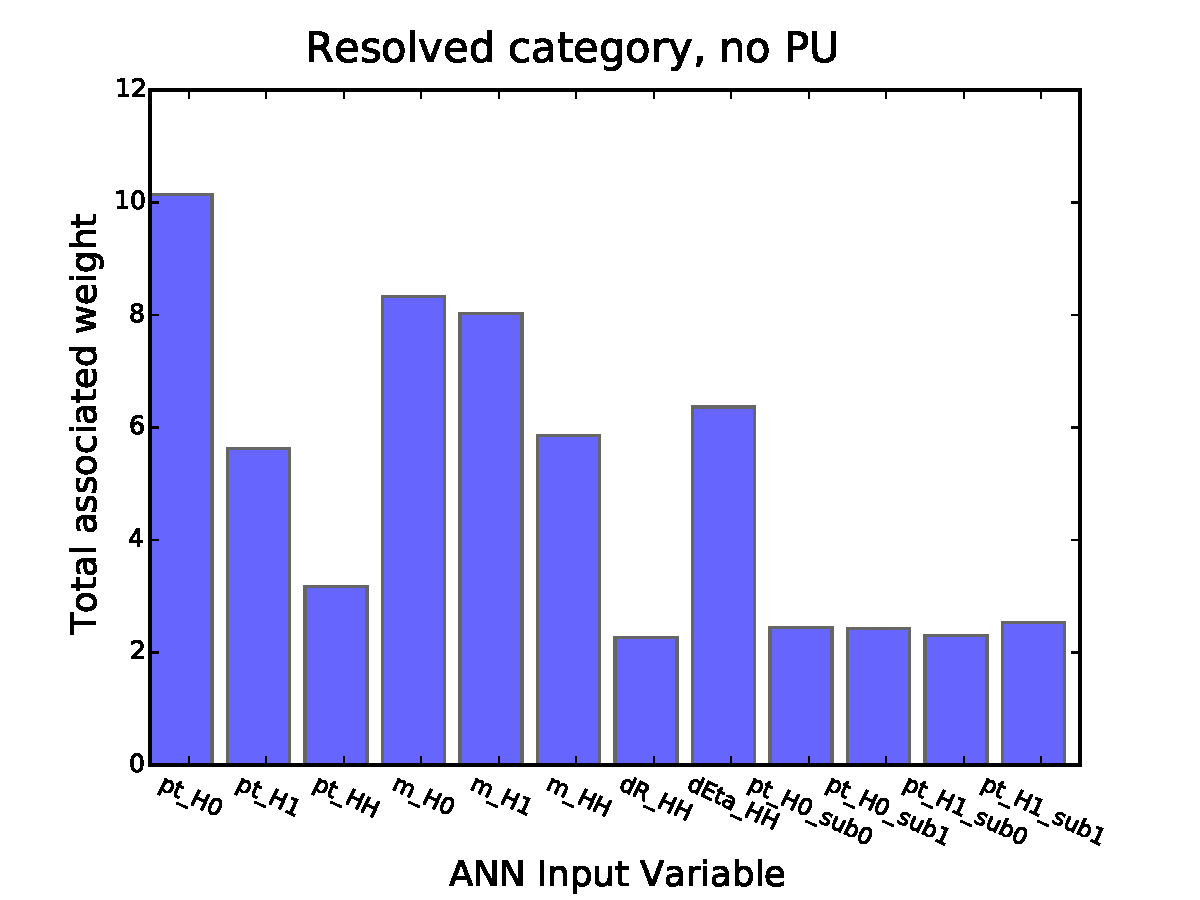
\includegraphics[width=0.49\textwidth]{plots/res_wgthist_noPU.pdf}
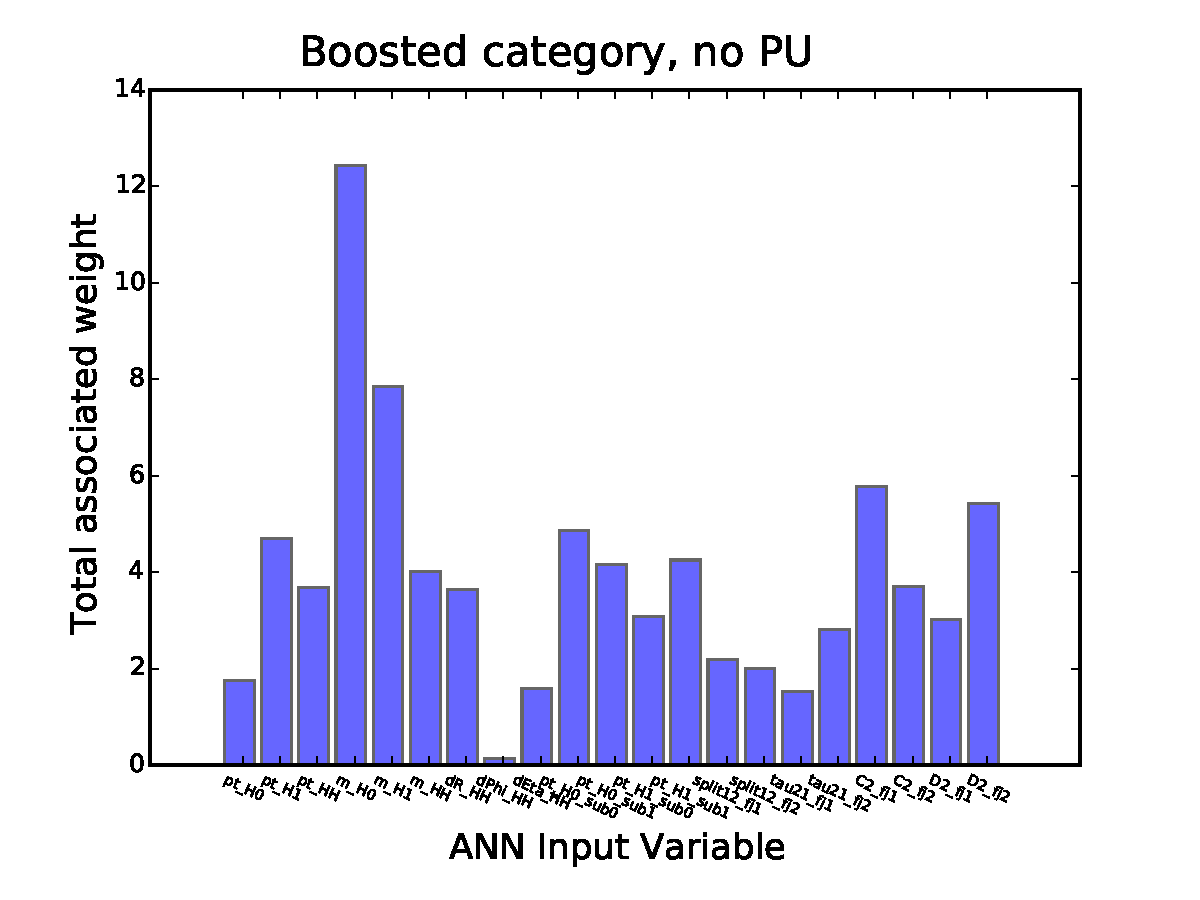
\includegraphics[width=0.49\textwidth]{plots/bst_wgthist_noPU.pdf}
\vspace{-0.5cm}
\caption{\small
Distribution of the total associated weight,
Eq.~(\ref{eq:totweight}) for each of the $N_{\rm var}$ input
variables of the resolved (left plot) and boosted (right plot) categories.
%
See Sect.~\ref{sec:input} for a description of each of the input
variables to the MVA.
}
\label{fig:nnweights}
\end{center}
\end{figure}
%%%%%%%%%%%%%%%%%%%%%%%




For the boosted category, we see that substructure variables
are the most helpful ones, in particular the $k_t$-splitting scale
$\sqrt{d_{12}}$ and the subjettiness ratio $\tau_{12}$.
%
The ratios of ECFs $D_2^{(\beta)}$ and
$C_2^{(\beta)}$ also seems to provide
useful discrimination power.
%
Concerning other kinematic variables, the angular
separation between the two large-$R$ jets $\Delta R_{hh}$,
the invariant mass of the di-Higgs system $m_{hh}$ and the various
$p_T$ also have discrimination power.
%
Other variables provide limited information, in particular the invariant
mass of the Higgs candidates, $m_{h_1}$ and $m_{h_2}$: this
is due to the realistic
simulation of detector resolution introduced with the smearing.
%
We have verified that the post-MVA
signal significance in the boosted category is substantially
degraded if substructure variables are not used.

At this point we have all the ingredients that we need to determine the optimal
value of the MVA output cuts $y_{\rm cut}$
and quantify the final values of the signal
significance $S/\sqrt{B}$ and $S/B$ in the three categories.
%
These optimal values are determined from the maximisation of $S/\sqrt{B}$,
ensuring that the number of events $N_{\rm ev}$
which would be expected at the HL-LHC is large
enough.
%
In addition, we also require when fixing $y_{\rm cut}$
that the actual number of MC events used for the ANN training
is large enough to avoid the biases of a small training sample.

These results are summarized in Table~\ref{table:cutflowMVA}, where we indicate
the value of the optimal ANN output
cut in each category,
the number of signal and background events $N_{\rm ev}$ expected
at the HL-LHC,
and also $S/\sqrt{B}$ and $S/B$.
%
For reference, we also include the results at the end of
the cut-based
analysis.
%

%%%%%%%%%%%%%%%%%%%%%%%%%%%%%%%%%%%%%%%%%%%%%%%%%%%%%%%%%%%%%%%%%%%%%%%%%%%%
%%%%%%%%%%%%%%%%%%%%%%%%%%%%%%%%%%%%%%%%%%%%%%%%%%%%%%%%%%%%%%%%%%%%%%%%%%%%
\begin{table}[t]
  \centering
  \begin{tabular}{|c|l|c|c|c|c|}
    \hline
    Category  &   &  $N_{\rm ev}$ signal &  $N_{\rm ev}$ back  &  $S/\sqrt{B}$ & $S/B$ \\ 
    \hline
    \hline
    \multirow{2}{*}{Boosted} &  $y_{\rm cut}=0$  & 1070 & $7.6\cdot 10^5$  & 1.2  & $1.4\cdot 10^{-3}$  \\
    &  $y_{\rm cut}=0.82$ & 790  & $2.2\cdot 10^4$   & 5.4  & 0.034 \\
    \hline
    \hline
    \multirow{2}{*}{Intermediate} &  $y_{\rm cut}=0$  & 670   & $5.3\cdot 10^5$
    & 0.9 & $1.2\cdot 10^{-3}$ \\
    &  $y_{\rm cut}=0.80$ & 360  & $5.5\cdot 10^3$  & 4.8 & 0.06\\
    \hline
    \hline
      \multirow{2}{*}{Resolved} &  $y_{\rm cut}=0$  & 3700 &  $1.5\cdot 10^{7}$ &  1.0 &$3\cdot 10^{-4}$ \\
    &  $y_{\rm cut}=0.65$ & 1300  & $8.3\cdot 10^{4}$ & 4.5 & 0.01 \\
    \hline
      \end{tabular}
  \caption{\small Post-MVA results, for the optimal value of the
    ANN discriminant $y_{\rm cut}$ in the three categories, compared with the
    corresponding
    pre-MVA results $y_{\rm cut}=0$.
    %
    We indicate the number of signal and
    background events
    at the HL-LHC with $\mathcal{L}=3$ ab$^{-1}$,
    the signal significance $S/\sqrt{B}$ and
    the signal over background ratio $S/B$.
    %
    The pre-MVA results ($y_{\rm cut}=0$) corresponds to row C2 in
    Table~\ref{tab:cutflow_noPU_1}.
    \label{table:cutflowMVA}
  }
\end{table}
%%%%%%%%%%%%%%%%%%%%%%%%%%%%%%%%%%%%%%%%%%%%%%%%%%%%%%%%%%%%%%%%%%%%%%%%%%%%
%%%%%%%%%%%%%%%%%%%%%%%%%%%%%%%%%%%%%%%%%%%%%%%%%%%%%%%%%%%%%%%%%%%%%%%%%%%%

The post-MVA results for $S/\sqrt{B}$ and $S/B$ as a function of the cut
in the ANN output for each of the three categories are shown in
Fig.~\ref{fig:sb_mva}.
%
Note that the values of $S/\sqrt{B}$ and $S/B$
for $y_{\rm cut}=0$ correspond to the values at
the end of the cut-based analysis, see
the C2 row of Table~\ref{tab:cutflow_noPU_1}.
%
Indeed, at the end of the cut based analysis, the
signal significance $S/\sqrt{B}$ was
1.2, 0.9 and 1.0 for the boosted, intermediate and resolved
categories respectively, consistent with Fig.~\ref{fig:sb_mva}.
%
The same applies to the signal over background ratio $S/B$.

%%%%%%%%%%%%%%%%%%%%%%%%
\begin{figure}[t]
\begin{center}
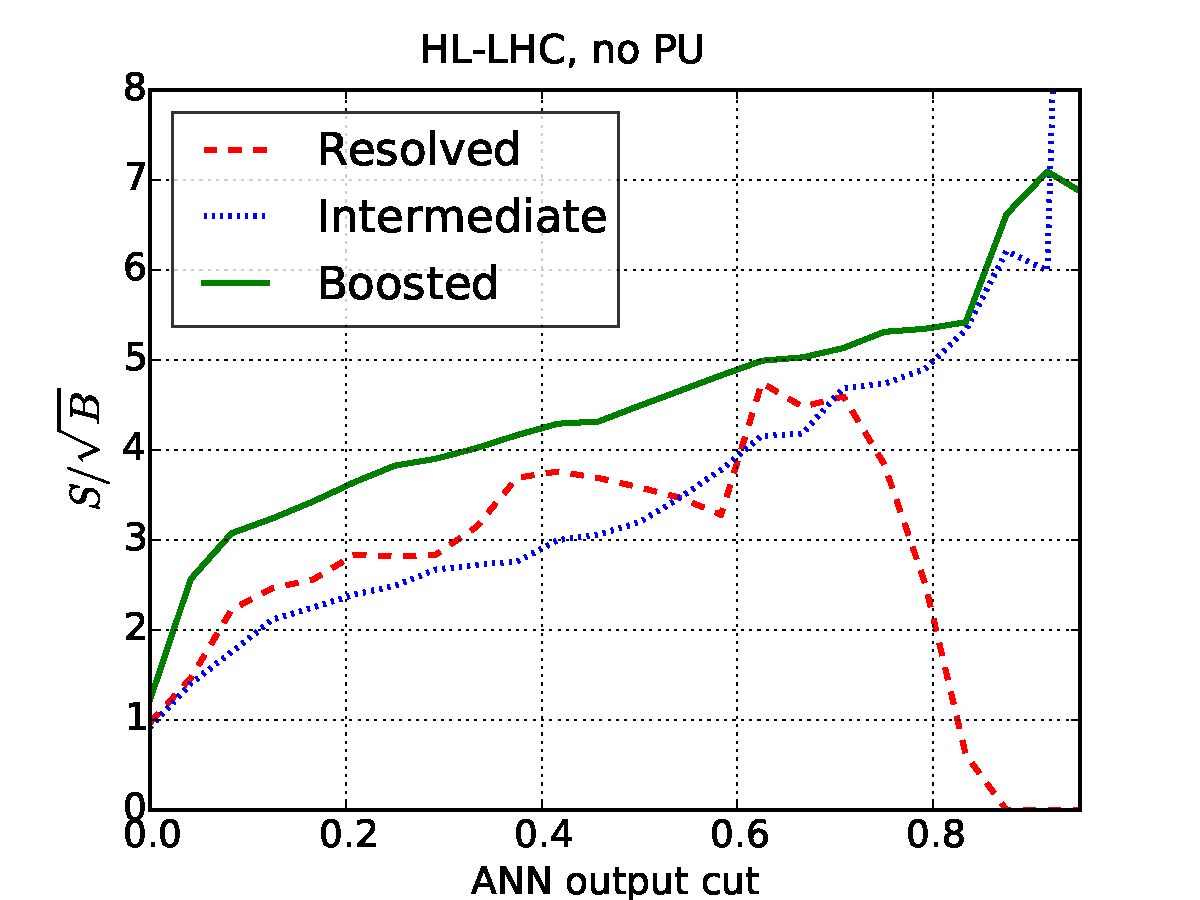
\includegraphics[width=0.48\textwidth]{plots/ssb_noPU.pdf}
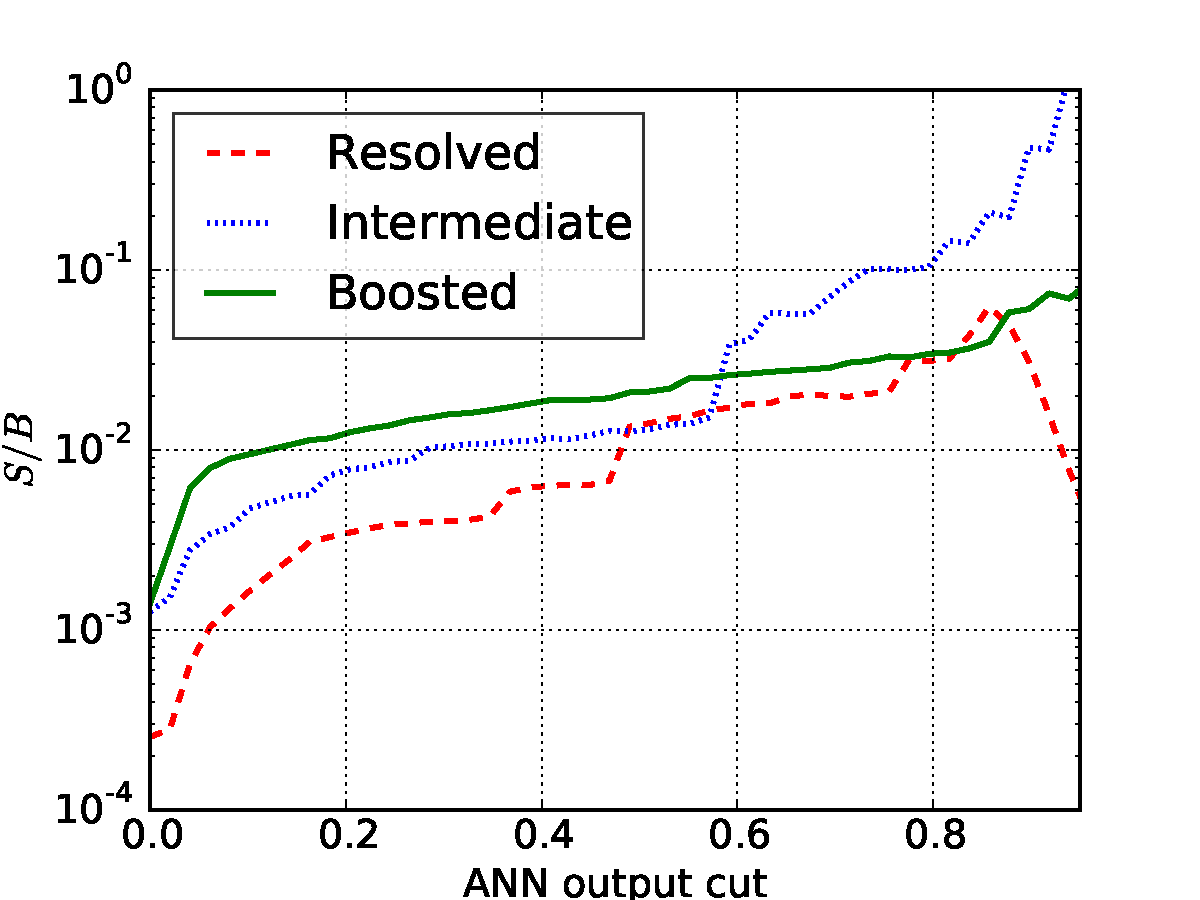
\includegraphics[width=0.48\textwidth]{plots/sb_noPU.pdf}
\caption{\small
  The values of the signal significance $S/\sqrt{B}$ and of the
  signal over background ratio $S/B$ for the boosted, intermediate
  and resolved categories as  function of the cut
  $y_{\rm cut}=0$ in the ANN output.
  %
  The $y_{\rm cut}=0$
  values correspond to the  cut-based analysis
  results from Table~\ref{tab:cutflow_noPU_1}.
}
\label{fig:sb_mva}
\end{center}
\end{figure}
%%%%%%%%%%%%%%%%%%%%%%%

The results of Fig.~\ref{fig:sb_mva}  show that
for all categories the  improvement in signal
significance arising from the MVA is substantial, growing from around 1
to around 5 in the three cases.
%
The optimal values of $y_{\rm cut}$ ensure that the
number of events at the HL-LHC is still well appreciable: we obtain
1300, 360 and 800 events in the resolved, intermediate, and
boosted categories respectively.
%
Another important benefit of the MVA applied to the boosted
category is that fact that the background is substantially
reduced so that $S/B$ can be as large as 10\% for the optimal
values of the ANN output cut.
%
Note that this is not true for the other two categories,
where $S/B$ is roughly constant.
%
A reasonably large value of $S/B$ is beneficial
from the experimental point of view, since it indicates
that the measurement is feasible even if the
systematic uncertainties are not very small.



From Table~\ref{table:cutflowMVA} we see that after the
MVA the signal significance in the boosted category increases
from 0.99 to 3.31, with $S/B$ increasing from $0.005$ to $0.10$,
with still more that 100 signal events at the HL-LHC.
%
Table~\ref{table:cutflowMVA} also shows that for the intermediate
and resolved categories, the improvement due to the use
of the MVA is rather moderate, and signal significance is always
small since backgrounds are still  large.
%
The combination of the signal significance of the
three categories leads to a $S/\sqrt{B}=3.53$, and compared
to 3.31 using only the boosted category.


Table~\ref{fig:sb_mva} contains the main result of this paper:
at the HL-LHC, it should be possible to claim evidence of
Higgs pair production using only the $4b$ final state.
%
Needless to say, to claim discovery and to improve the accuracy
of the measurement of the trilinear coupling it would still
be needed to combine this channel with others like
$b\bar{b}\gamma\gamma$ and $b\bar{b}\tau\tau$, but in any case
it is always important to have robust evidence from
individual channels.

These remarkable results are however subject to an obvious criticism:
at the HL-LHC the intense PU is know to substantially affect
kinematical distributions, and in particular, it is expected to degrade
in some extent the results of the present analysis.
%
To preempt this criticism, in the next section
we discuss how the expectations for the HL-LHC
summarized in  Table~\ref{fig:sb_mva} are modified in the presence
of PU expected at the HL-LHC.
%
But before that let us illustrate how the improvement in $S/\sqrt{B}$
obtained from the MVA in the boosted
category arises from the information contained in the
jet substructure variables.

\subsection{Another look at jet substructure variables}

%
From the distribution of total associated ANN weights in the
boosted category, shown in Fig.~\ref{fig:nnweights}, we see that
all substructure variables contain useful information:
the $k_t$-splitting scales $\sqrt{d_{12}}$,
the $\tau_{21}$ subjettiness ratio, and the ECF ratios
$C_2^{(\beta)}$ and $D_2^{(\beta)}$.
%
Interestingly, for some substructure variables, such as $\tau_{21}$,
the total associated weight turns out to be stronger in the leading
than in the sub-leading Higgs candidate (or vice-versa), indicating some
degree of redundancy when the same variable is used for the two Higgs candidates
at the same time.


The information reflected in Fig.~\ref{fig:nnweights} should also be
apparent from the corresponding distributions of these substructure
variables: those with a higher discrimination power should show
clear differences in shape between the signal and background events,
while those that carry less information should have similar
shapes for signal and background.
%
The third possibility is that of of redundant variables, where signal
and background exhibit different shapes but the same information
is already provided by other input variables.
%
To illustrate these points,
in Fig.~\ref{fig:mva_substructure_1}
we show the distributions of some of
these substructure variables for the boosted category: the
$k_t$ splitting scale $\sqrt{d_{12}}$, Eq.~(\ref{eq:ktsplitting}), for
the subleading Higgs,
the energy correlation double ratio $D_2^{(\beta)}$,
Eq.~(\ref{eq:d2}), for the leading Higgs,
and then 
the subjettiness ratio $\tau_{12}$,
Eq.~(\ref{eq:tau21}),
for both the leading and subleading Higgs candidates.
%

%%%%%%%%%%%%%%%%%%%%%%%%%%%%%%%%%%%%%%%%%%%%%%%%%%%%%%%
\begin{figure}[t]
  \begin{center}
    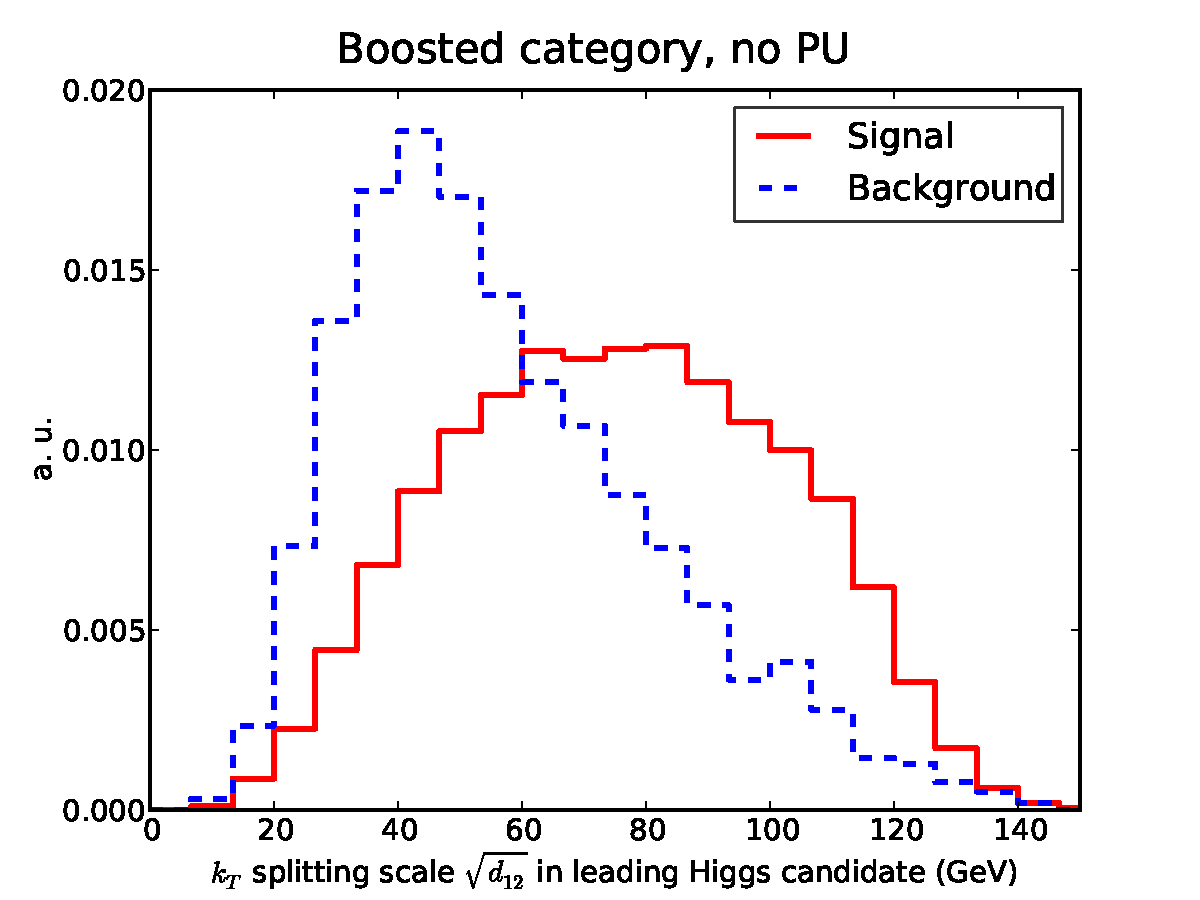
\includegraphics[width=0.48\textwidth]{plots/split12_h1_C1_boost.pdf} 
  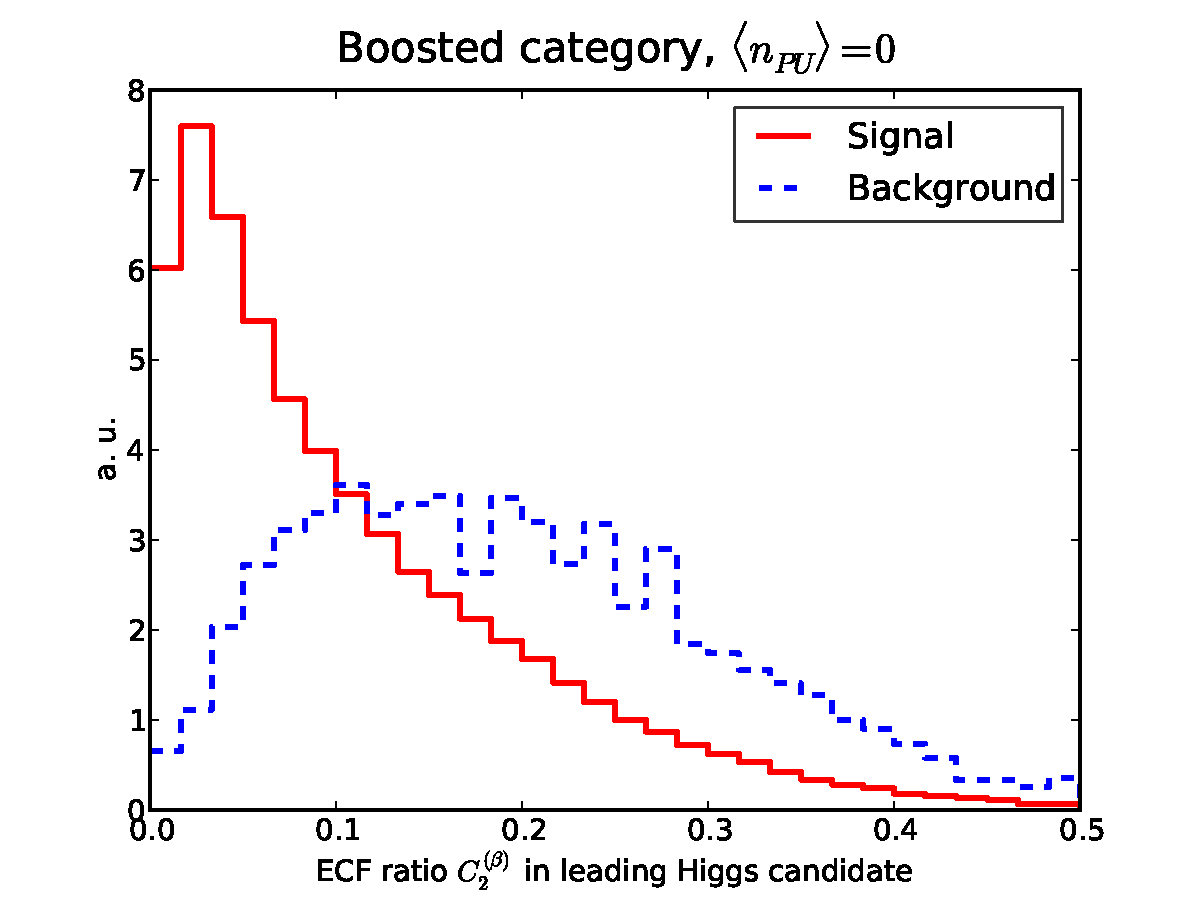
\includegraphics[width=0.48\textwidth]{plots/EEC_C2_h0_C1_boost.pdf}
  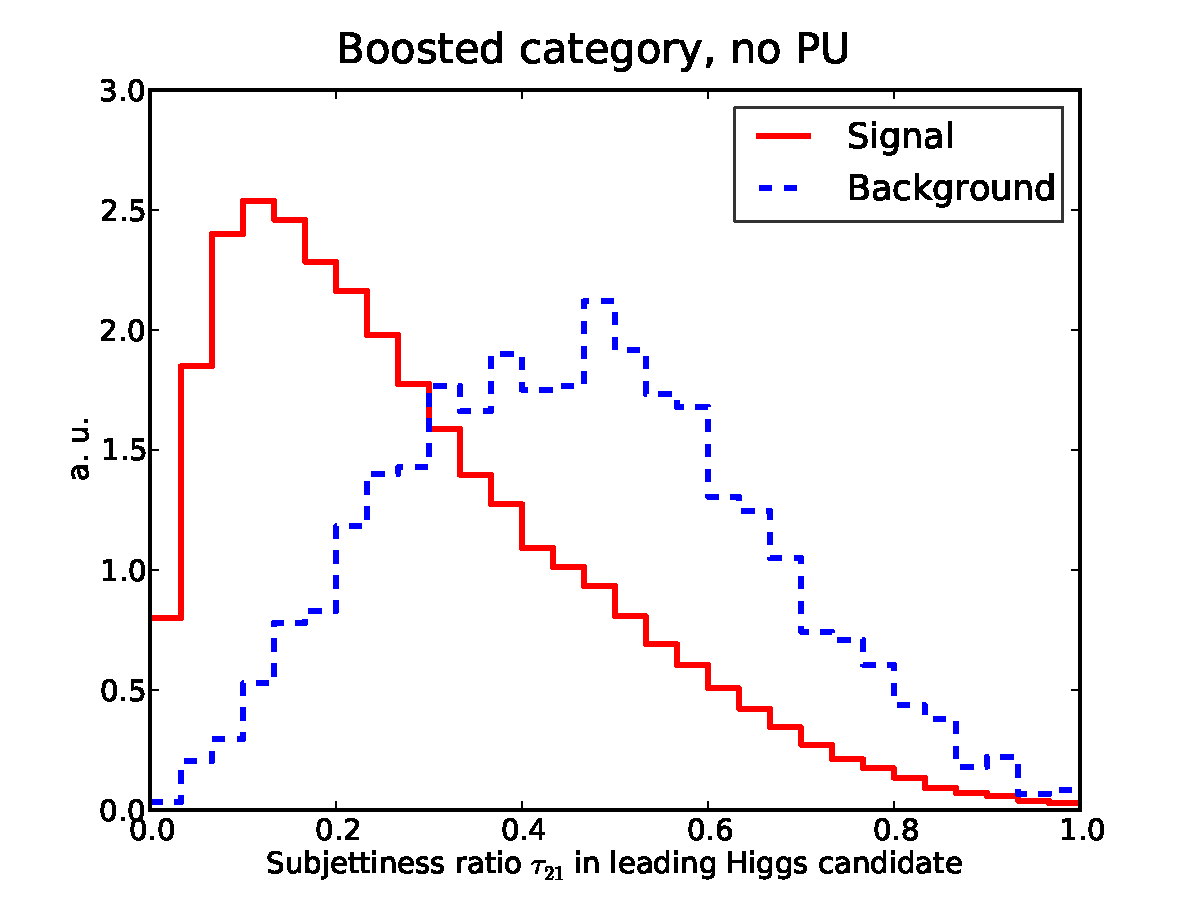
\includegraphics[width=0.48\textwidth]{plots/tau21_h0_C1_boost.pdf}
  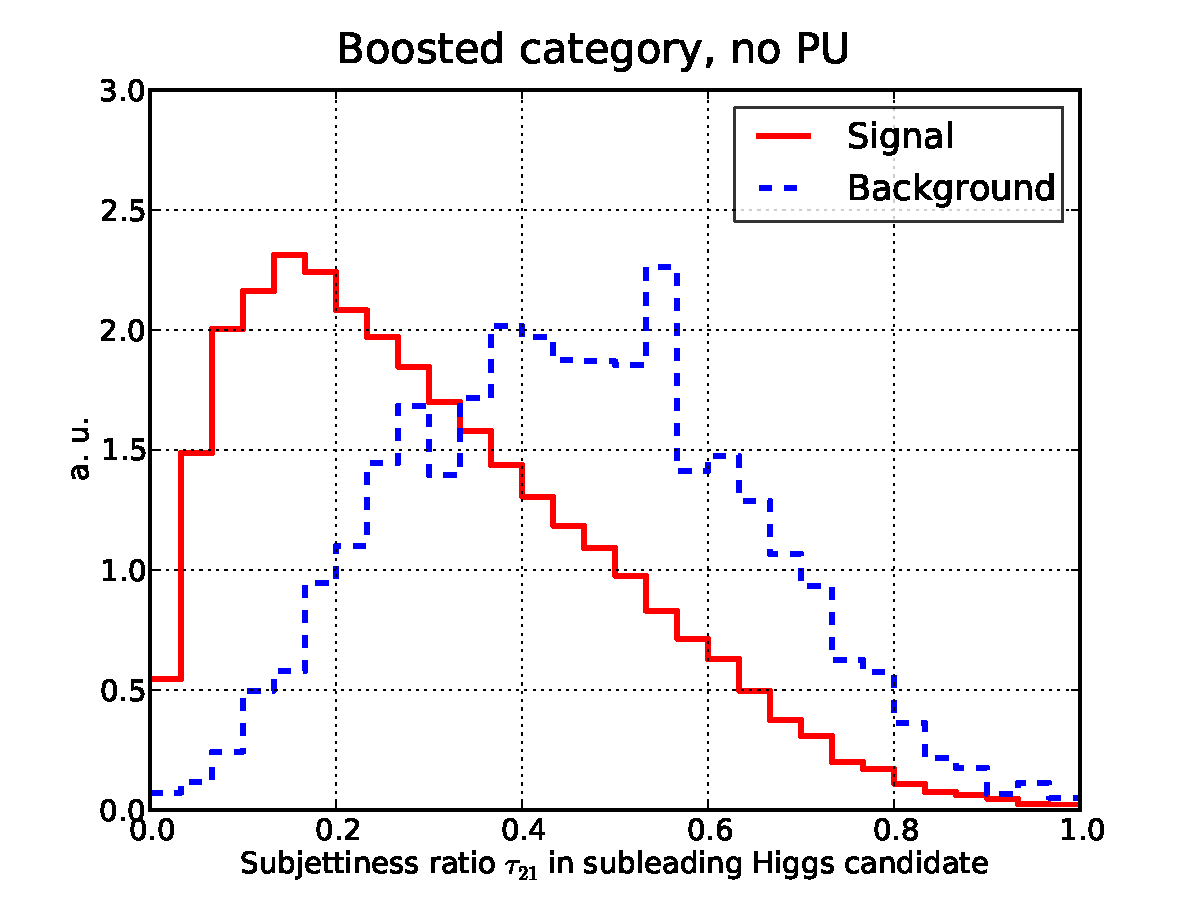
\includegraphics[width=0.48\textwidth]{plots/tau21_h1_C1_boost.pdf}
  \caption{\small Distribution of substructure variables
    in the boosted category at the end of the cut-based
    analysis, used as input to the MVA.
    %
    From top to bottom and from left to right we show  the
$k_t$ splitting scale for
the subleading Higgs, the subjettiness ratio $\tau_{12}$
for the leading Higgs,
and the energy correlation double ratio $D_2$
for the leading and subleading Higgs.
%
All distributions have been normalized to unity.
}
\label{fig:mva_substructure_1}
\end{center}
\end{figure}
%%%%%%%%%%%%%%%%%%%%%%%%%%%%%%%%%%%%%%%%%%%%%%%%%%%%%%%%%%%%%%%%%%%


From Fig.~\ref{fig:mva_substructure_1}
we can observe that for these substructure variables the shapes of the signal
and background distributions show important differences,
reflecting the inherent differences in the internal structure of jets
between QCD jets and jets originated from the Higgs decays.
%
Importantly, we observe that signal and background distributions peak
in different regions: for example, the $k_t$ splitting scale $\sqrt{d_{12}}$
peaks around 80 GeV (50 GeV) for signal (background) events, while
the ECF ratio $D_2^{(\beta)}$ peaks at much lower values for signal than
for background events.
%
From Fig.~\ref{fig:mva_substructure_1} we also see
the distributions of the subjettiness ratio $\tau_{12}$ are quite similar
in the leading and in the subleading jets, therefore adding
$\tau_{12}$ from the two Higgs candidates to the MVA at the same time
is redundant, explaining why in these cases either one or the other
variable from a Higgs candidate is assigned higher weight.


It is also interesting to show the distributions of kinematic variables
that according to the MVA provide a small amount of discrimination
between signal and background, and where the should not be an issue
of redundancy.
%
In Fig.~\ref{fig:mva_substructure_2}
we show the kinematic variable that carries less weight in the MVA,
    the azimuthal angle separation between the two Higgs candidates
    $\Delta\phi_{hh}$, for the resolved and boosted categories:
    according to Fig.~\ref{fig:nnweights}, essentially no discrimination power
    should be obtained from this variable, and indeed the shapes of the two signal
    and background
    are very similar here.
    %
    From Fig.~\ref{fig:nnweights} we also saw that the
    invariant mass distributions $m_h$ carry little information
    to discriminate signal over background:
    this was already verified from 
the corresponding
distributions in Fig.~\ref{fig:mHHinv}.
%
As explained before, the reduced discrimination power arises
from 
the  smearing of jet four-momenta introduced to mimic
realistically detector resolution.

%%%%%%%%%%%%%%%%%%%%%%%%%%%%%%%%%%%%%%%%%%%%%%%%%%%%%%%
\begin{figure}[t]
  \begin{center}
  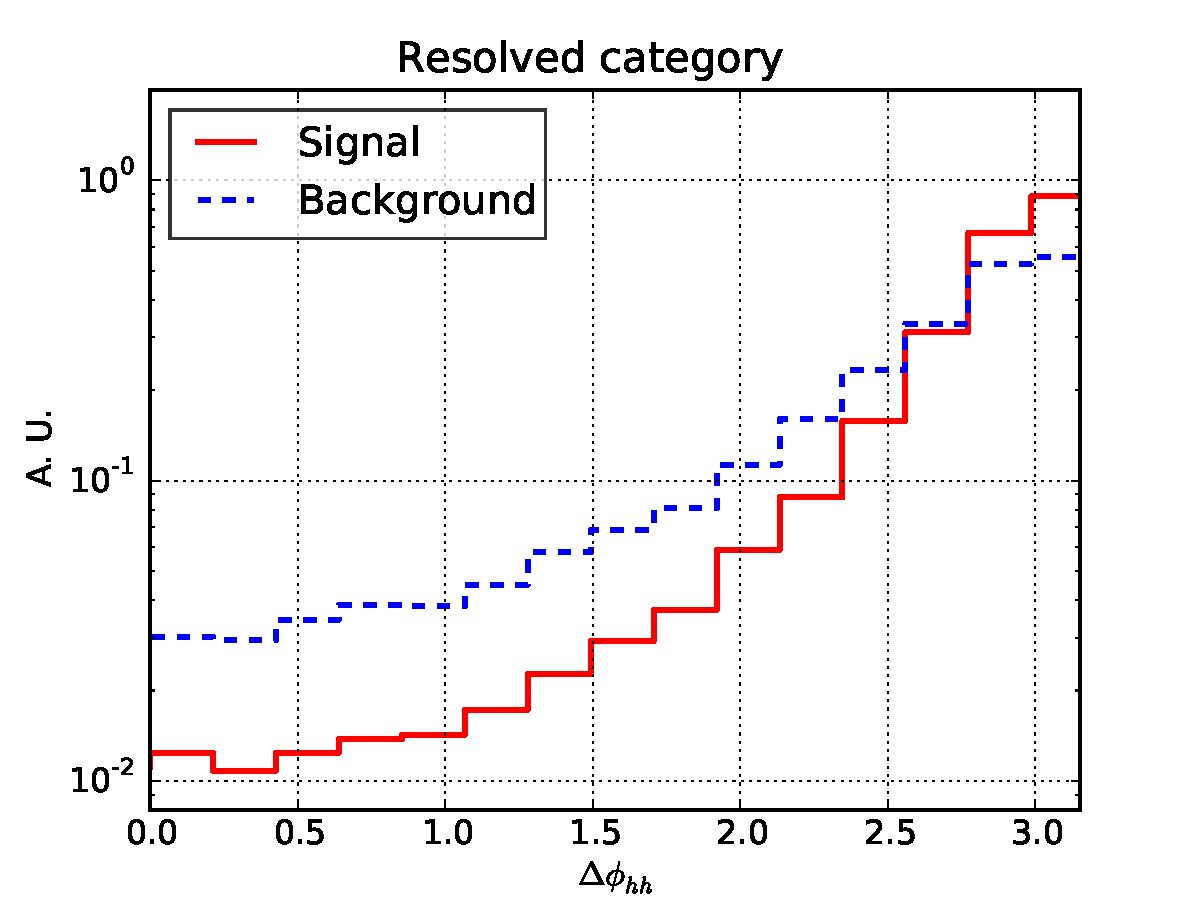
\includegraphics[width=0.48\textwidth]{plots/DeltaPhi_HH_C1_res.pdf} 
  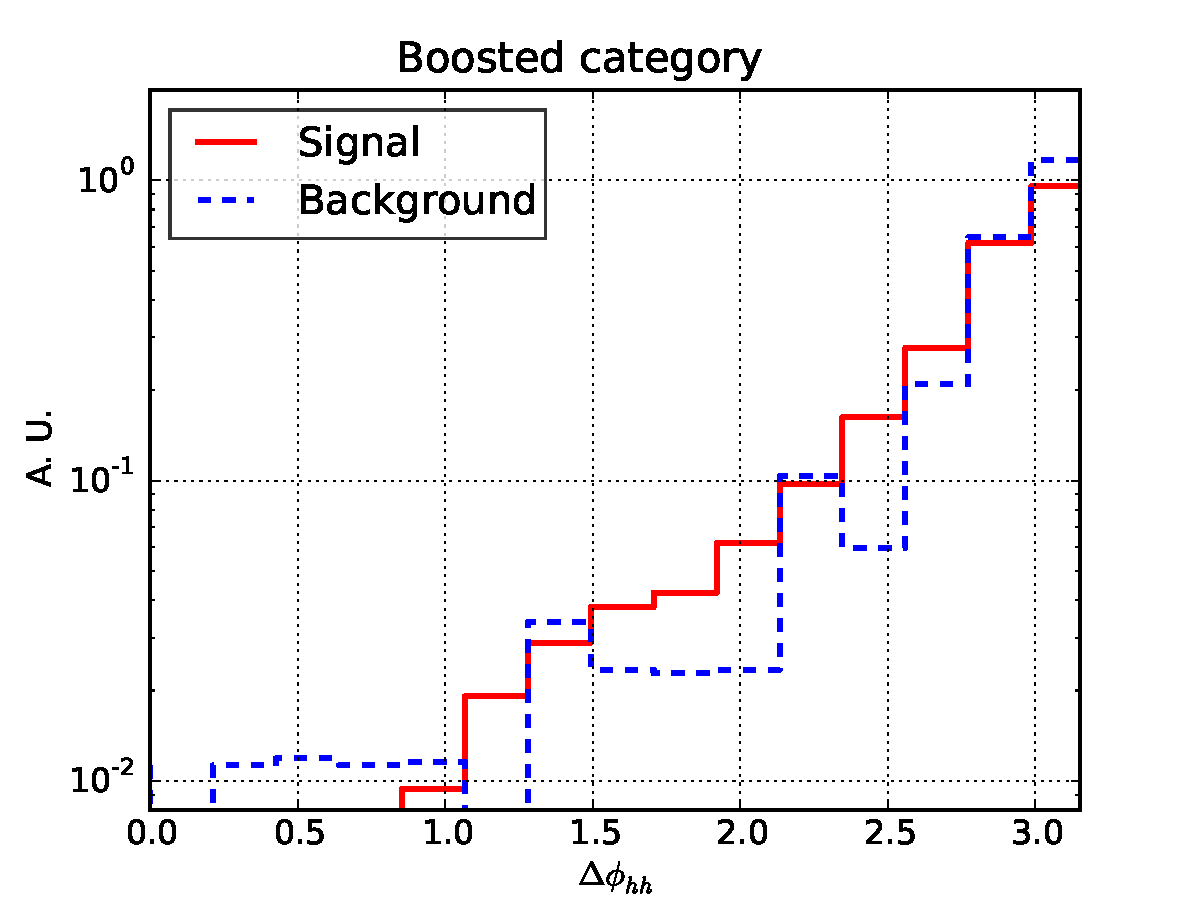
\includegraphics[width=0.48\textwidth]{plots/DeltaPhi_HH_C1_boosted.pdf} 
  \caption{\small Same as Fig.~\ref{fig:mva_substructure_1},
    now for the kinematic variable that carries less weight in the MVA,
    the azimuthal angle separation between the two Higgs candidates
    $\Delta\phi_{hh}$, for the resolved and boosted categories.
}
\label{fig:mva_substructure_2}
\end{center}
\end{figure}
%%%%%%%%%%%%%%%%%%%%%%%%%%%%%%%%%%%%%%%%%%%%%%%%%%%%%%%%%%%%%%%%%%%

\subsection{Impact of PU}

The main limitation of our analysis so far is the fact that
pile-up (PU) effects have not been accounted for
not accounted for.
%
However, any realistic feasibility study at the HL-LHC, specially
one 
such the present that relies on the careful modeling
of kinematic distributions,
requires assessing the robustness of the conclusions
with respect to the inclusion of PU.
%
In this section, we show how our qualitative results, in particular
the enhanced signal significance provided by the MVA, are robust
in the presence of  PU.


First of all, we describe the simulation of the 
PU conditions  expected at the HL-LHC, and discuss the settings of
the PU subtraction strategy that we adopt.
%
Then we present the validation of the PU subtraction,
and compare a number of distributions, including substructure variables,
with and without PU.
%
Finally we revisit the MVA analysis of Sect.~\ref{sec:mva}, and
show that our qualitative conclusions are robust
in the presence of realistic PU conditions, finding
a combined
signal significance of $S/\sqrt{B}\simeq 4$.


The same settings of the cut-based analysis,
Sects.~\ref{sec:analysis} and~\ref{sec:results}, and
the subsequent MVA optimization, Sect.~\ref{sec:mva}, have
been applied to the samples with PU, $\la n_{\rm PU}\ra=80$,
and SK subtraction.
%
The corresponding version of Table~\ref{tab:cutflow_noPU_1}, the 
cut-flow for the cross-sections and signal significance at the various
steps of the cut-based analysis, 
in the case
of PU subtracted with SK, for $\la n_{\rm PU}\ra=80$,
is presented in Table~\ref{tab:cutflow_SKPU80_1}.
%
One immediate observation is that
at the end of the cut-based analysis,
the signal significance have been  degraded
as compared to the case without PU.
%
We now obtain values for $S\sqrt{B}$ of 0.4, 0.3 and 0.9, in the resolved,
intermediate and boosted categories, respectively, to be compared
with the corresponding values without PU, namely 1.6, 1.6 and 2.7.
%
Therefore, the pre-MVA signal significance is degraded by a factor 4 in
the resolved and the intermediate categories,
and by a factor 3 in the boosted category.
%
The fact that the latter is the  least affected one
can be understood from the previous comparison
plots, which show that effects of PU contamination
are milder due to the  selection requirements
of the boosted category.

%%%%%%%%%%%%%%%%%%%%%%%%%%%%%%%%%%%%%%%%%%%%%%%%%%%%%%%%%%%
\begin{table}[t]
  \centering
  \scriptsize
  \begin{tabular}{|l|cc|cccc|cccc|}
  \hline
\multicolumn{11}{|c|}{Resolved category, $\la n_{\rm PU}\ra=80$+SK}\\
\hline
&  \multicolumn{6}{c|}{Cross-section [pb]} &  &  & &  \\
   &  $hh\to 4b$ &  total bkg  &   $4b$    &  $2b2j$   &   $4j$    &
$t\bar{t}$ &
$S/B_{\rm tot}$ & $S/B_{\rm 4b}$ & $S/\sqrt{B_{\rm tot}}$ & $S\sqrt{B_{\rm 4b}}$ \\
  \hline
  \hline
 C0    & 16  &   $3.1\cdot 10^9$   & $9.0\cdot 10^5$ & $2.1\cdot 10^8$ & $2.9\cdot 10^9$ & $1.8\cdot 10^5$ &   $5.0\cdot 10^{-9}$   & $1.7\cdot 10^{-5}$ &   $1.5\cdot 10^{-2}$   & 0.9 \\
 C1a   & 16  &   $3.1\cdot 10^9$   & $9.0\cdot 10^5$ & $2.1\cdot 10^8$ & $2.9\cdot 10^9$ & $1.8\cdot 10^5$ &   $5.0\cdot 10^{-9}$   & $1.7\cdot 10^{-5}$  &   $1.5\cdot 10^{-2}$   & 0.9 \\
 C1c   & 13  &   $1.1\cdot 10^9$   & $2.5\cdot 10^5$ & $7.7\cdot 10^7$ & $1.1\cdot 10^9$ & $1.3\cdot 10^5$ &   $1.1\cdot 10^{-8}$   & $5.3\cdot 10^{-5}$  &   $2.1\cdot 10^{-2}$   & 1.4  \\
 C1d   & 13 &   $1.1\cdot 10^9 $  & $2.5\cdot 10^5$ & $7.7\cdot 10^7$ & $1.1\cdot 10^9$ & $1.3\cdot 10^5$  &   $1.1\cdot 10^{-8}$   & $5.3\cdot 10^{-5}$  &   $2.1\cdot 10^{-2}$   & 1.4\\
 C1e   & 1.3  &   $3.9\cdot 10^7$   & $1.2\cdot 10^4$ & $2.8\cdot 10^6$ & $3.6\cdot 10^7$ & $3.3\cdot 10^4$  &   $3.4\cdot 10^{-8}$   & $1.1\cdot 10^{-4}$ &   $1.2\cdot 10^{-2}$   & 0.6\\
 C2    & 0.22  &   $2.3\cdot 10^3$   & $7.4\cdot 10^2$ & $1.4\cdot 10^3$ & $9.9\cdot 10^1$ & $1.6\cdot 10^1$  &   $9.8\cdot 10^{-5}$   & $3.0\cdot 10^{-4}$  &  $0.25$   & 0.4 \\
\hline
\end{tabular}

  $\,$ \\
  \vspace{0.5cm}
  \begin{tabular}{|l|cc|cccc|cccc|}
  \hline
\multicolumn{11}{|c|}{Intermediate category}\\
\hline
&  \multicolumn{6}{c|}{Cross-section [pb]} &  &  & &  \\
   &  $hh\to 4b$ &  total bkg  &   $4b$    &  $2b2j$   &   $4j$    &
$t\bar{t}$ &
$S/B_{\rm tot}$ & $S/B_{\rm 4b}$ & $S/\sqrt{B_{\rm tot}}$ & $S\sqrt{B_{\rm 4b}}$ \\
  \hline
  \hline
C0      & 16  &   $3.1\cdot 10^9$   & $9.0\cdot 10^5$ &  $2.1\cdot 10^8$ & $2.9\cdot 10^9$ & $1.8\cdot 10^5$ &   $5.0\cdot 10^{-9}$   & $1.7\cdot 10^{-5}$ &    $1.5\cdot 10^{-2}$   & 0.9\\
 C1b     & 6.1  &  $ 4.6\cdot 10^8$   &$ 1.6\cdot 10^5$ & $3.1\cdot 10^7$ & $4.3\cdot 10^8$ & $3.6\cdot 10^4$  &  $ 1.3\cdot 10^{-8}$   & $3.9\cdot 10^{-5}$  & $1.6\cdot 10^{-2}$   & 0.9 \\
 C1c     & 3.1  &   $8.7\cdot 10^7 $  & $2.4\cdot 10^4$ & $5.7\cdot 10^6$ & $8.1\cdot 10^7$ & $2.6\cdot 10^4$ &   $3.6\cdot 10^{-8}$   & $1.3\cdot 10^{-4}$ &  $1.8\cdot 10^{-2}$    & 1.1 \\ 
 C1d     & 3.2  &   $8.6\cdot 10^7 $  & $1.9\cdot 10^4$ & $5.6\cdot 10^6$ & $8.0\cdot 10^7$ & $2.4\cdot 10^4$  &   $3.7\cdot 10^{-8}$   & $1.7\cdot 10^{-4}$ &   $1.9\cdot 10^{-2}$   & 1.3 \\
 C1e     & 0.43  &   $2.7\cdot 10^7$   & $7.0\cdot 10^3$ & $1.8\cdot 10^6$ & $2.5\cdot 10^7$ & $9.3\cdot 10^3$  &   $1.6\cdot 10^{-8}$   & $6.2\cdot 10^{-5}$  &     $4.6\cdot 10^{-3}$   & 0.3 \\
 C2      & $3.2\cdot 10^{-2}$  &   $2.7\cdot 10^2$   & $3.7\cdot 10^1$ & $2.1\cdot 10^2$ & $1.8\cdot 10^1$ & 1.2 &  $ 1.2\cdot 10^{-4}$   & $8.6\cdot 10^{-4}$  &      0.1   & 0.3 \\
\hline
\end{tabular}

  $\,$ \\
  \vspace{0.5cm}
    \begin{tabular}{|l|cc|cccc|cccc|}
  \hline
\multicolumn{11}{|c|}{Boosted category, $\la n_{\rm PU}\ra=80$+SK}\\
\hline
&  \multicolumn{6}{c|}{Cross-section [pb]} &  &  & &  \\
   &  $hh\to 4b$ &  total bkg  &   $4b$    &  $2b2j$   &   $4j$    &
$t\bar{t}$ &
$S/B_{\rm tot}$ & $S/B_{\rm 4b}$ & $S/\sqrt{B_{\rm tot}}$ & $S\sqrt{B_{\rm 4b}}$ \\
  \hline
  \hline
 C0      & 16  &   $3.1\cdot 10^9$   & $9.0\cdot 10^5$ & $2.1\cdot 10^8$ & $2.9\cdot 10^9$ & $1.8\cdot 10^5$ &   $5.0\cdot 10^{-9}$   & $1.7\cdot 10^{-5}$  &   $1.5\cdot 10^{-2}$   & 0.9 \\
 C1a     & 16  &   $3.1\cdot 10^9 $  & $9.0\cdot 10^5$ & $2.1\cdot 10^8$ & $2.9\cdot 10^9$ & $1.8\cdot 10^5$ &   $5.0\cdot 10^{-9}$   & $1.7\cdot 10^{-5}$   &   $1.5\cdot 10^{-2}$   & 0.9 \\
 C1c     & 3.9  &   $4.7\cdot 10^8 $  & $8.9\cdot 10^3$ & $3.1\cdot 10^7$ & $4.3\cdot 10^8$ & $1.6\cdot 10^4$   &  $ 8.4\cdot 10^{-9}$   & $4.4\cdot 10^{-4}$  &  $ 9.9\cdot 10^{-3}$   & 2.3 \\
 C1d     & 2.7  &   $4.4\cdot 10^8 $  & $5.4\cdot 10^3$ & $2.9\cdot 10^7$ & $4.1\cdot 10^8$ & $1.3\cdot 10^4$ &   $6.0\cdot 10^{-9}$   & $5.0\cdot 10^{-4}$  &   $7.0\cdot 10^{-3}$   & 2.0 \\
 C1e     & 0.95  &   $1.1\cdot 10^7$   & $1.5\cdot 10^3$ & $7.0\cdot 10^5$ & $9.8\cdot 10^6$ & $4.7\cdot 10^3$  &  $ 9.1\cdot 10^{-8}$   & $6.4\cdot 10^{-4}$  &   $1.6\cdot 10^{-2}$   & 1.4 \\
 C2      & 0.11  &   $2.7\cdot 10^2$   & $4.2\cdot 10^1$ & $2.1\cdot 10^2$ & $1.1\cdot 10^1$ & $6.8\cdot 10^{-1}$  &  $ 4.0\cdot 10^{-4}$   & $2.5\cdot 10^{-3}$  &   $0.35$   & 0.9 \\
\hline
\end{tabular}

    \caption{\small
      Same as Table~\ref{tab:cutflow_noPU_1}, for the analysis
      including PU with $\la n_{\rm PU}\ra=80$ and SK subtraction.
      \label{tab:cutflow_SKPU80_1}}
\end{table}
%%%%%%%%%%%%%%%%%%%%%%%%%%%%%%%%%%%%%%%%%%%%%%%%%%%%%%%%%%


In Table~\ref{table:cutflowMVA_PU}
we provide the  the number of signal and
    background events expected
    at the HL-LHC, as well as the
    corresponding values for $S/\sqrt{B}$ and $S/B$,
    for both the cut-based analysis (corresponding
    to $y_{\rm cut}=0$) and after the
    optimal MVA cut, for the simulations
    with $\la n_{\rm PU}\ra=80$
    and SK subtraction.
    %
    The same results without PU are those of
    Table.~\ref{table:cutflowMVA}.
    %
    From Table~\ref{table:cutflowMVA_PU} we see that, thanks
to the MVA, we can improve the signal significance and the
signal over background ratio from 0.35 and $4\cdot 10^{-4}$
(0.25 and $1\cdot 10^{-4}$) up to 2.9 and 0.034 (2.5 and 0.15)
in the boosted (resolved) category.
%
The intermediate category exhibits a rather lower value of $S/\sqrt{B}$
for the optimal $y_{\rm cut}$ value, around 1.1.
%
We thus conclude that, as was already the case
without PU,
the boosted category is the most promising
one for the study of Higgs pair production in the $b\bar{b}b\bar{b}$
final state
at the HL-LHC, also when PU is included.
%
However, important information will also be obtained from
the resolved category, which has a signal significance
only slightly smaller than the boosted case.



%%%%%%%%%%%%%%%%%%%%%%%%%%%%%%%%%%%%%%%%%%%%%%%%%%%%%%%%%%%%%%%%%%%%%%%%%%%%
%%%%%%%%%%%%%%%%%%%%%%%%%%%%%%%%%%%%%%%%%%%%%%%%%%%%%%%%%%%%%%%%%%%%%%%%%%%%
\begin{table}[t]
  \centering
  \begin{tabular}{|c|l|c|c|c|c|}
    \hline
    Category  &   &  $N_{\rm ev}$ signal &  $N_{\rm ev}$ back  &  $S/\sqrt{B}$ & $S/B$ \\ 
    \hline
    \hline
    \multirow{2}{*}{Boosted} &  $y_{\rm cut}=0$  & 360   &  $1.4\cdot 10^6$ & 0.31   &
     $3\cdot 10^{-4}$  \\
    &  $y_{\rm cut}=0.82$ &  250 & 7300  & 2.9    & 0.034  \\
    \hline
    \hline
    \multirow{2}{*}{Intermediate} &  $y_{\rm cut}=0$  &  150  & $9\cdot 10^5$    & 0.15    &
     $2\cdot 10^{-4}$ \\
    &  $y_{\rm cut}=0.80$ & 50 & 2600  &  1.1   & 0.02 \\
    \hline
    \hline
    \multirow{2}{*}{Resolved} &  $y_{\rm cut}=0$  &  1100  & $8.5\cdot 10^6$
    & 0.25    &  $1.3\cdot 10^{-4}$  \\
    &  $y_{\rm cut}=0.65$ & 430  & $3\cdot 10^4$  &  2.5   & 0.15  \\
    \hline
      \end{tabular}
  \caption{\small Same as Table~\ref{table:cutflowMVA}, now for the case
    of PU+SK, with $\la n_{\rm PU}\ra=80$.
        \label{table:cutflowMVA_PU}
  }
\end{table}
%%%%%%%%%%%%%%%%%%%%%%%%%%%%%%%%%%%%%%%%%%%%%%%%%%%%%%%%%%%%%%%%%%%%%%%%%%%%
%%%%%%%%%%%%%%%%%%%%%%%%%%%%%%%%%%%%%%%%%%%%%%%%%%%%%%%%%%%%%%%%%%%%%%%%%%%%

Another important result from Table~\ref{table:cutflowMVA_PU} is that,
for the optimal MVA cut, the signal over background ratio
is not unfeasibly small: we obtain that $S/B$ is 3.4\% (1.5\%)
in the boosted (resolved) categories.
%
This is indicates that while this measurement is still very challenging,
requiring a careful extraction from the data of the QCD
background, it is certainty within reach.
%
Our analysis also indicates a possible way forward to
further increase $S/B$: reducing the background from light and charm
fakes, see Table~\ref{tab:cutflow_SKPU80_1}.

Let us now discuss in more detail the results of the MVA
classification, by showing various estimators as function
of the cut $y_{\rm cut}$ in the ANN discriminant.
%
In Fig.~\ref{fig:nev2_PU}
we show the number of signal and background events that
are expected at the HL-LHC as a function of
$y_{\rm cut}$ -
the corresponding results without PU are those of
Fig.~\ref{fig:nev2}.
%
As we can see, the general trends are
similar as those without PU.
%
Comparing Figs.~\ref{fig:nev2} and~\ref{fig:nev2_PU}, we also observe
that the intermediate category is substantially degraded once PU effects
are accounted for, the reason being  sizable
a reduction in the number of signal
events that are now assigned to this category.
%
This shows that the selection criteria
of the intermediate category are less
resilient against PU contamination,
as opposed to the resolved and boosted selections.

%%%%%%%%%%%%%%%%%%%%%%%%%%%%%%%%%%%%%%%%%%%%%
\begin{figure}[t]
\begin{center}
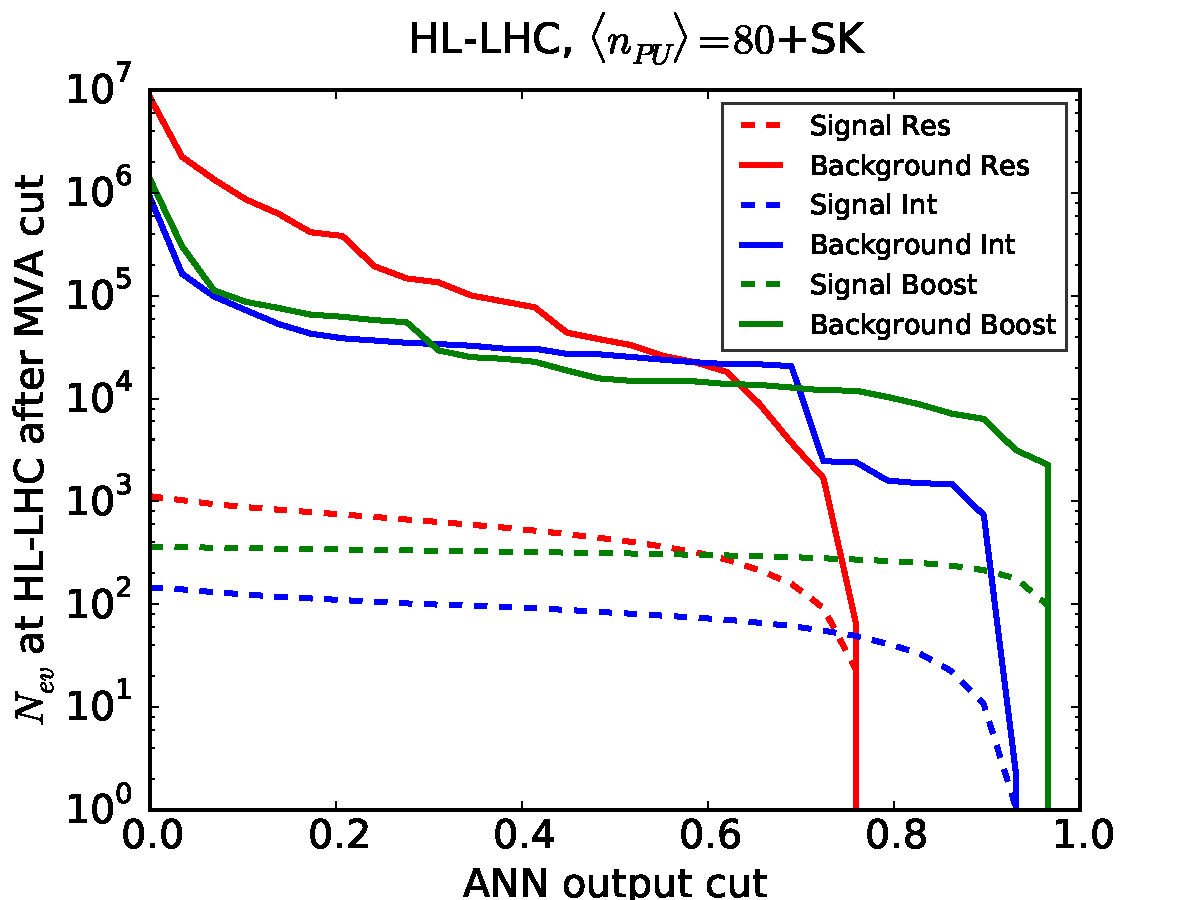
\includegraphics[width=0.65\textwidth]{plots/nev2_SKPU80.pdf}
\caption{\small Same as Fig.~\ref{fig:nev2} in the
case of events with PU, for
 $\la n_{\rm PU}\ra=80$ 
  and SK subtraction.
}
\label{fig:nev2_PU}
\end{center}
\end{figure}
%%%%%%%%%%%%%%%%%%%%%%%%%%%%%%%%%%%%%


In Fig.~\ref{fig:sb_mva_PU} we show the signal significance,
$S/\sqrt{B}$, as well as the signal over background ratio,
$S/B$, including now the effects of PU.
%
The corresponding results in the case without PU were shown in
Fig.~\ref{fig:sb_mva}.
%
As can be seen, the MVA-driven enhancement is robust in the
presence of PU.
%
While unsurprisingly there us a degradation as compared to the case wo PU,
we still manage to achieve a signal significance of
around $S/\sqrt{B}\simeq 2.5$ separately for the boosted and resolved
categories.
%
On the other hand, the intermediate category becomes irrelevant.
%
We conclude that the qualitative conclusions drawn in
Sect.~\ref{sec:mva} are robust in the presence
of realistic PU effects.
%
Since no specific effort has been performed to
optimize PU subtraction, for example by tuning the value
of the patch length $a$ in {\tt SoftKiller}, we believe that
there is
still room for improvement in this respect.


%%%%%%%%%%%%%%%%%%%%%%%%%%%%%%%%%%%%%%%%%%%%%%%%%%%%
%%%%%%%%%%%%%%%%%%%%%%%%%%%%%%%%%%%%%%%%%%%%%%%%%%%%
\begin{figure}[t]
\begin{center}
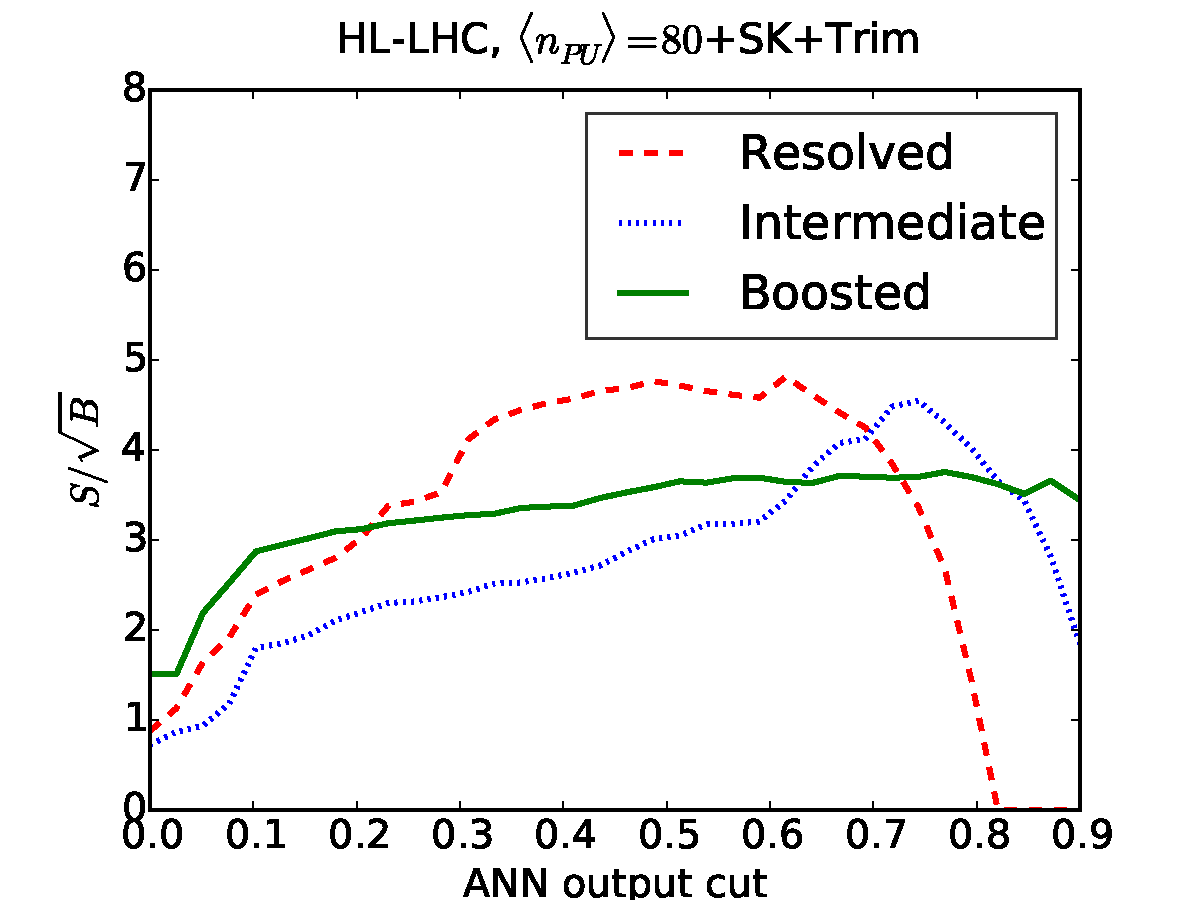
\includegraphics[width=0.48\textwidth]{plots/ssb_SKPU80.pdf}
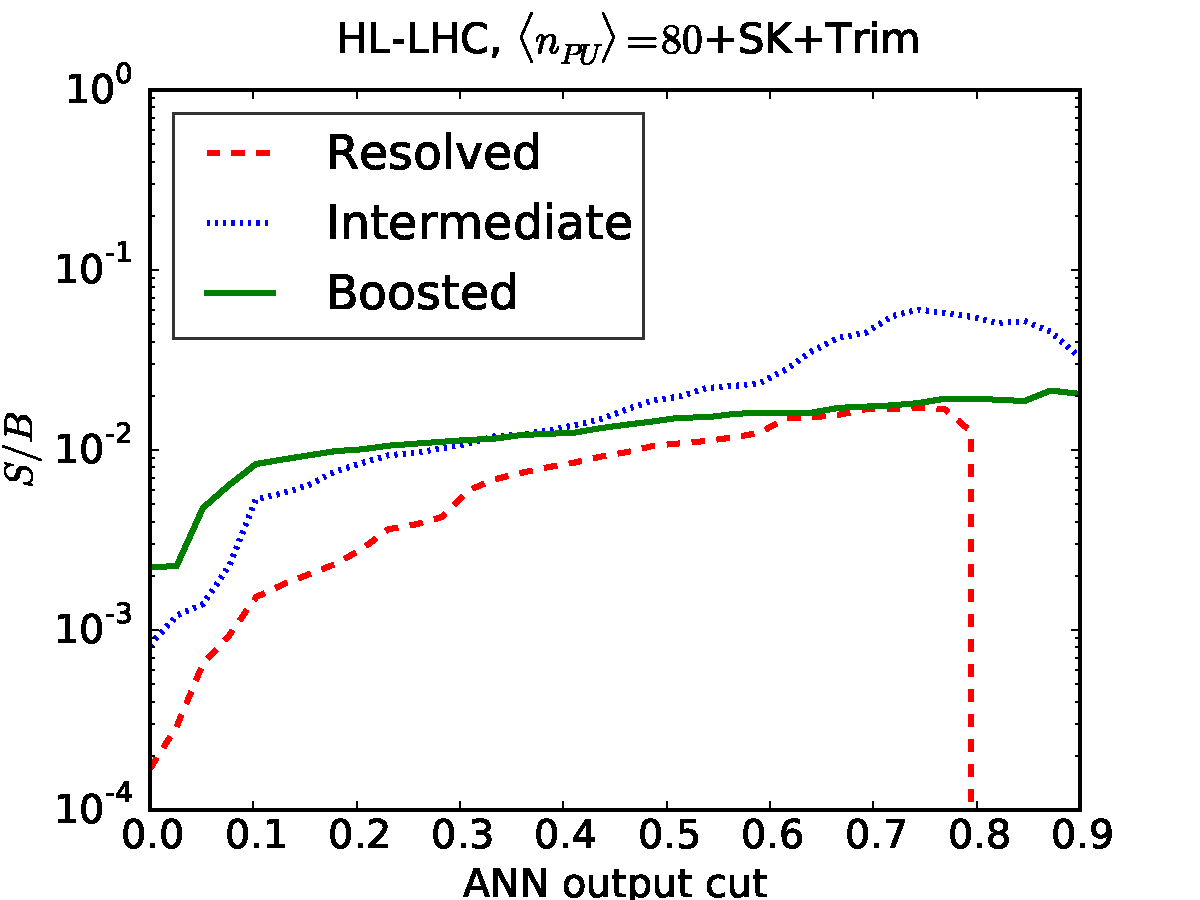
\includegraphics[width=0.48\textwidth]{plots/sb_SKPU80.pdf}
\caption{\small 
Same as Fig.~\ref{fig:sb_mva} in the
case of events with PU, for
 $\la n_{\rm PU}\ra=80$ 
  and SK subtraction.
}
\label{fig:sb_mva_PU}
\end{center}
\end{figure}
%%%%%%%%%%%%%%%%%%%%%%%

It is important to quantify which of the input variables
to the MVA carry the highest discrimination power
in the case of PU,
and compare it with the corresponding
results without PU.
%
We use the same estimator as in Sect.~\ref{sec:signalsignificance},
namely the sum
of the absolute value of all the weights connected to a given
input neuron $i$, Eq.~(\ref{eq:totweight}).
%
The results for the resolved and boosted categories are shown
on Fig.~\ref{fig:nnweights_PU}.
%
As we can see by comparing to the corresponding
results without PU in Fig.~\ref{fig:nnweights}, 
in the boosted category, the discrimination power of the invariant
mass of Higgs candidates is decreased and that of the various substructure
variables, in particular $C_2^{(\beta)}$ and
$D^{(\beta)}$, is conversely
increased.
%
This reflects the fact that these substructure variables are
relatively robust against PU contamination.
%
In addition, also the $p_T$ distributions of the AK03
subjets within the large-$R$
jets carry important information.
%
In the case of the resolved category,  the highest
values of the ANN weights without PU
were found for the $p_T$ of the leading
Higgs and for the Higgs invariant masses.
%
This is also true in the case with PU, but now the rapidity difference
between the two Higgs candidates, $\Delta y_{hh}$ increases its
importance, again reflecting that this variable is relatively
insensitive to PU effects.
%

%%%%%%%%%%%%%%%%%%%%%%%%
\begin{figure}[t]
\begin{center}
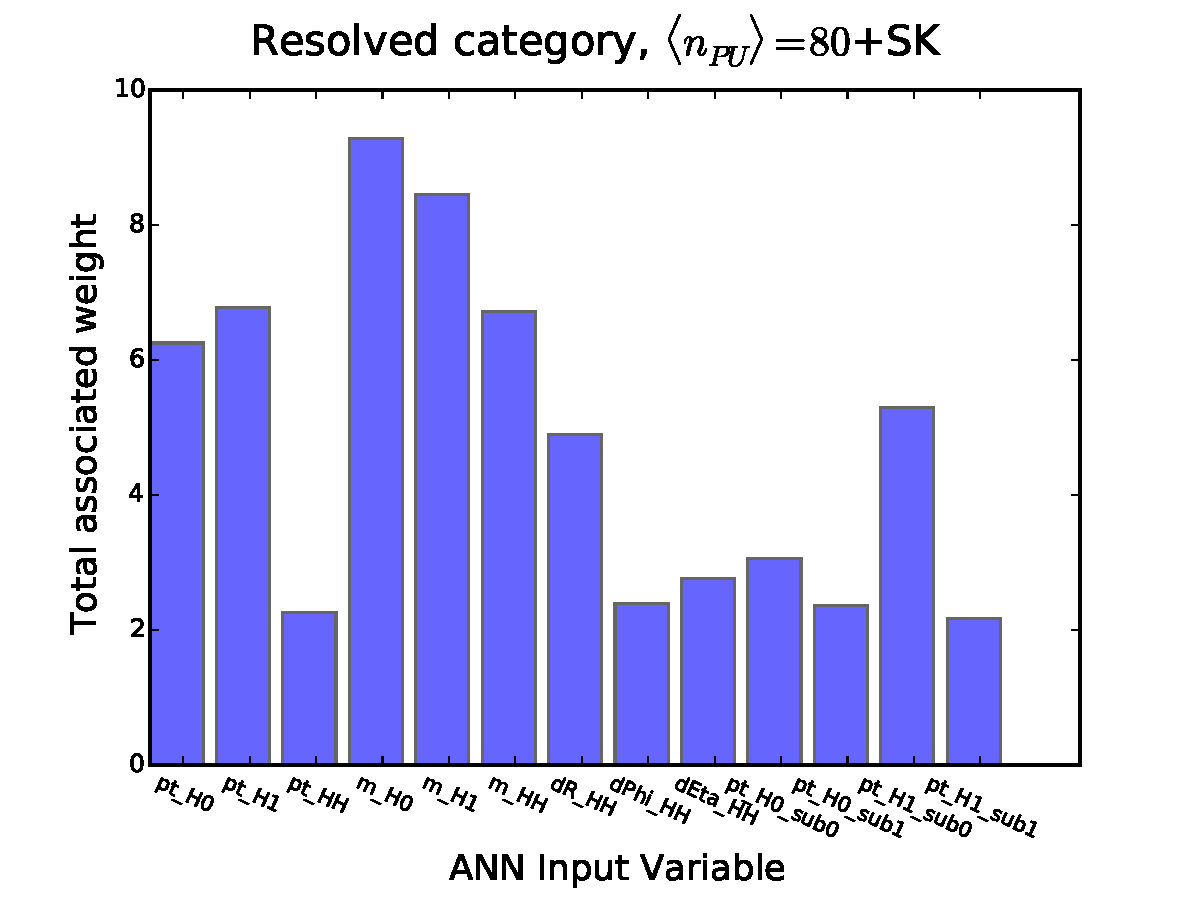
\includegraphics[width=0.49\textwidth]{plots/res_wgthist_SKPU80.pdf}
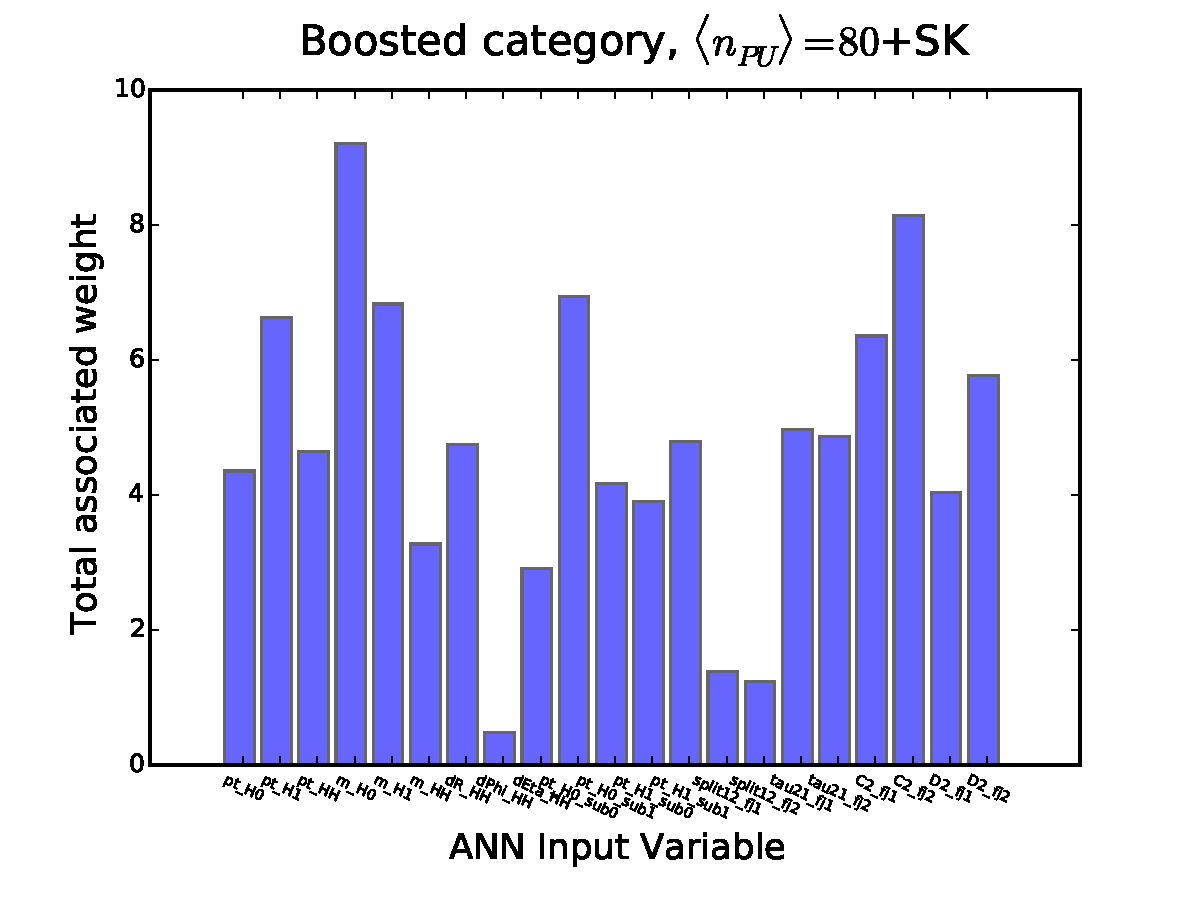
\includegraphics[width=0.49\textwidth]{plots/bst_wgthist_SKPU80.pdf}
\vspace{-0.5cm}
\caption{\small
Same as Fig.~\ref{fig:nnweights} in the
case of events with PU, for
 $\la n_{\rm PU}\ra=80$ 
  and SK subtraction.
}
\label{fig:nnweights_PU}
\end{center}
\end{figure}
%%%%%%%%%%%%%%%%%%%%%%%

At this point, we can finally combine the three categories, resolved,
intermediate and boosted, and determine the overall signal
significance taking into account all event topologies.
%
Adding in quadrature the signal significance from the three
(exclusive) categories for the corresponding
optimal value of $y_{\rm cut}$, our final combined result, accounting
for PU effects, is
\be
\lp \frac{S}{\sqrt{B}}\rp_{\rm tot} \simeq 4.0 \, ,
\ee
to be compared to the value $\lp S/\sqrt{B}\rp_{\rm tot} \simeq 8.5$
that was obtained in the case without PU.
%
We conclude that, even when realistic PU effects are accounted
for, at the HL-LHC the measurement of
Higgs pair production in the $b\bar{b}b\bar{b}$ final state should be 
well the threshold for evidence, and even meeting the
requirement for discovery might be within reach.
%

In summary, in this section we have demonstrated the robustness
of our results under the presence of PU conditions as those
expected at the HL-LHC.
%
With a signal significance of $S/\sqrt{B}\sim 4$, is clear that
the $b\bar{b}b\bar{b}$ final state can be used to claim evidence
for Higgs pair production at the HL-LHC without the need
to combine with any other final state.
%
Our analysis certainly contains
room for improvement, in particular by means of a tailored
study dedicated to optimize PU subtraction in this process.
%
It will be important now to quantify the precision of
a extraction of the Higgs trilinear coupling $\lambda$ using
the techniques presented here, but this is left for future work.

%%%%%%%%%%%%%%%%%%%%%%%%%%%%%%%%%%%%%%%%%%%%%%%%%%%%%%%%%%%%%%%%%%%%%%%%%%%%%%%%
%%%%%%%%%%%%%%%%%%%%%%%%%%%%%%%%%%%%%%%%%%%%%%%%%%%%%%%%%%%%%%%%%%%%%%%%%%%%%%%%
%%%%%%%%%%%%%%%%%%%%%%%%%%%%%%%%%%%%%%%%%%%%%%%%%%%%%%%%%%%%%%%%%%%%%%%%%%%%%%%%
%%%%%%%%%%%%%%%%%%%%%%%%%%%%%%%%%%%%%%%%%%%%%%%%%%%%%%%%%%%%%%%%%%%%%%%%%%%%%%%%
%%%%%%%%%%%%%%%%%%%%%%%%%%%%%%%%%%%%%%%%%%%%%%%%%%%%%%%%%%%%%%%%%%%%%%%%%%%%%%%%
